%=======================================================================
%  Attention Averages Where Convolution Adds : An Extensivity Dichotomy
%  Single column, 10pt, Times New Roman (newtx).
%  Build:  pdflatex paper.tex   (twice, for cross-references)
%  Blue text marks a blank the author still has to fill in: \needwrite{...}
%=======================================================================
\documentclass[10pt]{article}

\usepackage[T1]{fontenc}
\usepackage[margin=1.15in]{geometry}
\usepackage{amsmath,amssymb,amsthm}
\usepackage{newtxtext,newtxmath}   % Times New Roman text + matching Times math
\usepackage{graphicx}
\usepackage{booktabs}              % every table uses the same three-rule style
\usepackage{array}
\usepackage{caption}
\usepackage[section]{placeins}
\raggedbottom
\setcounter{topnumber}{2}
\setcounter{bottomnumber}{1}
\setcounter{totalnumber}{3}
\renewcommand{\topfraction}{0.85}
\renewcommand{\bottomfraction}{0.6}
\renewcommand{\textfraction}{0.12}
\renewcommand{\floatpagefraction}{0.75}
\usepackage{microtype}
\usepackage[title,titletoc]{appendix}
\usepackage{xcolor}
\usepackage{pgfplots}
\pgfplotsset{compat=1.18}
\usepgfplotslibrary{groupplots}
\usepgfplotslibrary{fillbetween}
\usepackage[hidelinks]{hyperref}   % links are live but printed in plain black
\hypersetup{
  pdftitle={Attention Averages Where Convolution Adds: An Extensivity Dichotomy},
  pdfauthor={Brayden Siew},
  pdfsubject={Transformer expressivity, counting, attention normalization}}
\usepackage[numbers,sort&compress]{natbib}

\captionsetup{font=small,labelfont=bf,labelsep=period,skip=6pt}
\setlength{\parskip}{0pt}
\renewcommand{\arraystretch}{1.15}

%=== theorem environments: upright body, bold heading, no italics =======
\theoremstyle{definition}
\newtheorem{theorem}{Theorem}
\newtheorem{lemma}{Lemma}
\newtheorem{corollary}{Corollary}
\newtheorem{conjecture}{Conjecture}
\newtheorem{definition}{Definition}
\newtheorem{example}{Example}
\newtheorem{remark}{Remark}

\makeatletter
\renewenvironment{proof}[1][\proofname]{\par\pushQED{\qed}\normalfont
  \topsep6\p@\@plus6\p@\relax\trivlist
  \item[\hskip\labelsep\bfseries #1\@addpunct{.}]\ignorespaces}
  {\popQED\endtrivlist\@endpefalse}
\makeatother

%=== shorthands =========================================================
\newcommand{\Inv}{\mathrm{Inv}}
\newcommand{\clampf}{\mathrm{clamp}}
\newcommand{\LN}{\mathrm{LN}}
\newcommand{\Cov}{\mathrm{Cov}}
\newcommand{\corr}{\mathrm{corr}}
% Blue = a blank only the author can fill. Every one must be gone before
% submission; grep for \needwrite to find them all.
\newcommand{\needwrite}[1]{\textcolor{blue}{[\,#1\,]}}

\title{\bfseries Attention Averages Where Convolution Adds\\[2pt]
\large An Extensivity Dichotomy}
\author{Brayden Siew}
\date{}

\begin{document}

\maketitle
\thispagestyle{empty}

\begin{abstract}
A softmax attention head averages the evidence it gathers, because its
weights always sum to one; a convolution adds. This paper shows that this
one difference decides whether a Transformer can output a count.

We study questions whose correct answers grow with input length, such as
how many items exceed a threshold or how many pairs of entries are out of
order. For fixed-depth Transformers with normalized attention and a fixed
single-pass readout, we prove that every output is confined to a range set
by the weights alone, independent of input length, so past a critical
length the correct count leaves the range the model can produce. For
inversion counting the unavoidable worst-case error grows quadratically
with length, and neither depth, width, positional encoding, attention
sharpness, nor numerical precision enters the bound. We then prove a
matching converse: a single additive attention head, keeping the query and
key comparison but replacing the normalized average with an un-normalized
sum, represents every counting question in this class exactly, at every
length.

Experiments support both halves. In a controlled toy the hand-constructed
head is exact at every length, and restoring only its denominator, with
every other weight held fixed, destroys it. A learned version of the head
on a frozen pretrained model extrapolates far past its training length and
answers counting questions never posed during training, while the standard
readouts do worse than ignoring the input. On a real document, a current
reasoning model in a single pass is worse than ignoring the input on
pairwise counts, and chain of thought restores correctness only at $29$ to
$4096$ times the output tokens. The practical conclusion is that these
failures are range errors, not reasoning errors, and one added head, which
provably never disturbs the original model, removes them.
\end{abstract}

\vspace{6pt}
\noindent\textbf{Keywords:} Transformer expressivity; softmax attention;
counting; length generalization; additive attention head; impossibility
result

\newpage
\setcounter{tocdepth}{1}
\tableofcontents
\newpage

%=======================================================================
\section{Introduction}
\label{sec:intro}
%=======================================================================

Give a language model a list of numbers and ask which one is largest, and
it will give you the right answer. However, if you ask how many pairs in
that same list are out of order, then past a certain length it stops
giving you the correct answer. Training it longer does not fix this, and
neither does making it larger. This
paper is about why the second question is different from the first.

The short answer is that it is arithmetic, not a training failure. A
softmax head returns $\sum_j w_j v_j$ with weights that are never negative
and always total one, so what comes out is an average of the values it
mixed. Layer normalization then pulls the state back to a fixed size at
every layer. Follow that through a fixed number of layers into a fixed
readout and the final number is trapped inside a box whose size is decided
by the model's own weights and by nothing else, certainly not by how long
the list is. Meanwhile the true count keeps growing. Once there are
more correct answers than the box has slots, two lists with different
answers have to come out the same, by the pigeonhole principle. Extra
precision buys nothing here, because the difficulty is not how finely the
model can write a number down. It is that the number it needs has stopped
being inside the range it can produce.

One comparison makes it click, and it is the reason
for the title. A convolution slides a kernel across its input and adds up
what it finds. Its weights are free, nobody makes them total anything, so
its output is allowed to grow. Attention slides a comparison across its
input and then averages what it finds, because its weights are forced to
total at most one. Those are the same shape of operation. The only thing
separating them is whether the last step divides.

If you sort operations by that one step, and by how the kernel gets
chosen, you get a small table with one interesting hole in it.

\begin{table}[htbp]
\centering
\caption{Where the additive head sits. The row is decided by the last
aggregation before the readout, whatever the architecture is called.}
\label{tab:twobytwo}
\begin{tabular}{@{}lll@{}}
\toprule
\textbf{Final aggregation} & \textbf{Kernel fixed by position} & \textbf{Kernel chosen by content} \\
\midrule
A sum & convolution with sum-pooling & the additive head in this paper \\
An average & convolution with average-pooling & softmax attention \\
\bottomrule
\end{tabular}
\end{table}

So the row is the thing that matters here, and the row is set by the last
aggregation before the readout, whatever the architecture is called. A
convolutional
network that finishes with global average pooling is in the bottom row and
has the same problem. Density-map crowd counting, which predicts a map and
then adds it up, is in the top row and does not. Attention is not worse
than convolution here. The difference is one step, and attention is the
only one of the four where nobody ever got to choose it. Normalization is what makes attention work
as a selector in the first place, so the averaging is not a decision
somebody made and could have made differently. It comes with the
mechanism, for free, whether you want it or not.

The table is a way of seeing one theorem. The bounded readout lemma below
covers the whole bottom row in one go.

That is the first of the two theorems, and we call it the extensivity
barrier. It applies to a whole family of questions at once. Fix any yes-or-no rule
you like, then ask how many items
in the list obey it, or how many pairs do. How many sevens. How many numbers above two. How many
duplicate pairs. All of them grow with the list, and all of them are
blocked for the same reason. What is not blocked is the yes-or-no twin of
each question, ``is there at least one'', because that answer stays $0$ or
$1$ forever and fits in the box easily. Attention is fine at deciding
which. It is the how many that breaks.

The second theorem says one head is enough to fix it. Keep the query and
key comparison, since comparing pairs is what attention is already good
at, and throw away the denominator. Put a clamp on each comparison so it
comes out as a clean vote, zero or one, then add the votes on a private
wire that runs to the readout without being squashed on the way. It is a
sidecar bolted to the motorcycle, not a new motorcycle. One of these
covers every question in the family because any yes-or-no rule over a
finite alphabet is just a table of zeros and ones, and a table of zeros
and ones is something a query and key product reproduces exactly. We write
the weights down by hand with linear algebra. No training, no gradient
descent, so no failure can be blamed on the optimizer.

Put the two together and what we get is that zero additive heads are enough
for none of these questions, and one is enough for all of them.

Then we go and check it, first in a toy we built, where an ablation ladder
changes one thing at a time. Normal attention fails out of range. Sharper
attention fails. A deeper and wider model fails. Then we take our own
working head, put the denominator back, change nothing else, and the
failure returns, which is the experiment that identifies the cause. Then on a real pretrained model, Qwen3-0.6B,
frozen, where only the small head reading its features changes. If the
additive head does better there it cannot be because it had a better
language model underneath, since all three heads read exactly the same
frozen vectors. We also run a model roughly seven times larger, to answer
the obvious objection that the small one simply lacked capacity. It does
not move the wall.

The hand-built construction is exact, the learned version is approximate
in ways we measure, and Section~\ref{sec:limits} says exactly where the
learned results stop.

In summary, the paper contributes:
\begin{enumerate}
\item The Extensivity Barrier (Theorem~\ref{thm:barrier}): no fixed-depth
  Transformer with normalized attention and a single-pass readout can emit
  any item or pair count that grows with input length, and for inversions
  the worst-case error grows quadratically. Depth, width, precision, and
  attention sharpness do not appear in the bound.
\item One-head universality (Theorem~\ref{thm:universal}): a single
  clamp-gated additive head with hand-constructed weights computes every
  counting question in the class exactly, at every length, giving the
  zero-versus-one dichotomy of Corollary~\ref{cor:zeroone}.
\item Validation at three scales: a controlled toy whose denominator
  ablation isolates normalization as the cause, learned heads on a frozen
  pretrained model that extrapolate in length and transfer to questions
  never used in training, and a real-document comparison against a
  reasoning model that prices the standard workaround.
\end{enumerate}

Section~\ref{sec:related} places the result against the work that got
close first.

%=======================================================================
\section{Related Work}
\label{sec:related}
%=======================================================================

Prior work falls into four areas: what each aggregator can represent, what
Transformers can and cannot count, formal limits on soft attention, and
the known ways around those limits. A final subsection states exactly
where this paper differs from the three closest results.

\paragraph{Aggregators and what they preserve.}

Deep Sets \citep{zaheer2017deepsets} shows that every permutation-invariant
set function can be written $\rho(\sum_i \phi(x_i))$; the result is proved
for countable universes or fixed-size sets, so for growing inputs we use it
as intuition and not as a citation of record. The sharper statement for our
purposes comes from graph networks \citep{xu2019gin}: sum preserves the
full multiset, mean only the proportions, max only the support, so a mean
cannot tell a set from the same set repeated. That failure is what an inability to count looks like.

\paragraph{Transformers and counting.}

\citet{yehudai2024count} prove the sharpest learnability limit: once the
vocabulary exceeds the embedding dimension, token embeddings interfere and
the weights needed for exact counting grow polynomially, so counting
becomes practically unlearnable even though solutions exist.
\citet{chang2024counting} argue that inductive counting needs an explicit
architectural bias and does not arrive with scale. On the mechanistic side,
\citet{golkar2024contextual} find that a model trained on contextual
counting implements a sum with the beginning-of-sequence token as its bias
term, although that sum still sits inside a softmax, and
\citet{cagnetta2024small} identify softmax normalization as what blocks a
counter subspace at fixed length. \citet{salzer2026counting} characterize
counting expressivity formally, and \citet{yang2024counting} give C-RASP,
the tightest known lower bound for soft attention. Both concern counts
\emph{compared} inside the network; neither addresses the count being
\emph{emitted}, and that is the question here. \citet{zhang2024tokenization} show that tokenization alone moves counting
accuracy substantially, which is why our experiments use single digits
with clean token boundaries.

\paragraph{Formal limits on soft attention.}

\citet{hahn2020} shows that a single input token can move a soft-attention
output by only $O(1/n)$. His parity result is easy to overstate: for soft
attention it bounds confidence, with cross-entropy converging to chance,
and the flat impossibility holds only for hard attention.
\citet{chiang2022} then construct a Transformer that recognizes parity
exactly by scaling the logits with $\log n$, and \citet{salzer2026counting}
agree from the expressivity side. That $\log n$ repair is the intervention
most likely to be mistaken for a fix here, and it is not one: it sharpens
the attention distribution, while our barrier concerns the range of the
output, and the $\log n$-scaled baseline in Section~\ref{sec:ablation}
fails exactly as Theorem~\ref{thm:barrier} predicts. \citet{merrill2023}
place log-precision Transformers in $\mathsf{TC}^0$, and \citet{sanford2023}
prove the pairwise detection bound that Section~\ref{sec:dichotomy} builds
on. All of these bound a computational class. Ours bounds a numerical
range, and it survives unbounded precision and width, which is why extra
decimal places do not help.

\paragraph{Softmax normalization, kept and removed.}

\citet{richter2020cage} prove the geometry this paper starts from: softmax
weights are nonnegative and sum to one, so every head output stays inside
the convex hull of its value vectors. They name it the probability cage and
conjecture, without proving, that it has consequences. Two results describe
how selection then degrades with length: with bounded logits every
attention coefficient is $\Theta(1/n)$ \citep{velickovic2024softmax}, and
once the selected set grows in proportion to the sequence, the separation
between selected and ignored must collapse \citep{mudarisov2025norm}.
\citet{barbero2024glasses} describe the over-squashing side of the same
picture and state in prose the claim nearest to ours. Lowering the softmax
temperature escapes none of this, since it only changes which values
receive the weight while the weights still sum to one. Two systems papers
remove softmax for engineering reasons: sigmoid attention with a $-\log n$
bias \citep{ramapuram2024sigmoid}, and ReLU attention with a $1/L$ scale
\citep{wortsman2023relu}. Both reintroduce an explicit length factor, so
neither is a clean escape from a bounded output; what they establish for
our purposes is that removing the normalization is an ordinary engineering
step.

\paragraph{Escapes and length generalization.}

Chain of thought is a genuine escape, and Theorem~\ref{thm:barrier} does
not touch it. Without intermediate tokens a Transformer sits in
$\mathsf{TC}^0$ \citep{merrill2023}; with them, logarithmic step budgets
reach $\mathsf{L}$, linear budgets cover the regular languages, and
polynomial budgets give exactly $\mathsf{P}$ \citep{merrill2023cot}, up to
Turing completeness over a unary alphabet \citep{turing2025cot}.
\citet{dziri2023faith} supply the practical counterweight: on large
compositional problems models skip items and propagate early mistakes,
which is also what our real-document experiment prices out. On length
generalization, \citet{huang2024lengthgen} give conditions under which
short training transfers to long inputs, but their formalism fixes the
answer alphabet at inference, and for how-many questions the answer set
itself grows with $n$; that reading is ours, not a limitation they concede.
\citet{izzo2025lengthgen} bound the training length that suffices, not what
fails below it.

\subsection{Where this paper sits}
\label{sec:related-position}

Three papers come close enough to require an exact statement of the
difference. \citet{ouellette2023counting} come closest. They ``point out
that applying a softmax operation over the attention weights makes it
impossible to learn to count entities across the input tokens in a parallel
manner'', and they close by writing that ``further research is needed to
determine the extent of this phenomenon, and to better understand it''.
What they establish is empirical and about learning: removing softmax and
layer normalization from a one-layer encoder lets unary grid counting
generalize far beyond the training range. \citet{cagnetta2024small} find
the same blockage mechanistically, at fixed length.
\citet{garcia2026direction} approach it from the readout instead: the count
is present in the hidden states, recoverable by a linear probe at $R^2$
above $0.99$, but stored along a direction nearly orthogonal to the output
head's digit rows, and a low-rank correction on the query and value weights
recovers $83.1\%$ greedy-generation accuracy.

The mechanism, then, is not new, and this paper does not claim it is. What
this paper adds is the extent that \citet{ouellette2023counting} asked for.
First, the statement covers the whole class of item and pair counting
questions at once, not only token-level unary counts. Second, it is proved
as an impossibility, for every parameter setting and every fixed depth,
with no assumption about precision, which makes it a fact about
representation rather than about learning. Third, it comes with a converse
over the same class, with weights written by hand instead of trained, which
turns the impossibility into a dichotomy and lets the escape list in
Table~\ref{tab:escapes} be complete rather than merely suggestive.

The distinction that matters most is with \citet{garcia2026direction},
since the two papers look at the same wall from opposite sides. They locate
the problem in the readout \emph{direction}, and routing can be re-aimed,
which is why their fix works as well as it does. We locate it in the
readout \emph{range}, and re-aiming cannot help with range, because inside
a bounded set no direction points at an unbounded number. Both can be true
at once, and Conjecture~\ref{conj:readout} is our attempt at saying how
they fit together.

\section{Preliminaries}
\label{sec:prelim}
\begin{remark}[No positional encoding is required]
\label{rem:nope}
We do not need to add positional encoding for this, because at position
$i$ the attention may look only at earlier positions $j < i$, and for
GPT-style models the attention is already causal and enforces this rule:
it looks at the token itself and the tokens before it.
\end{remark}

%=======================================================================

\subsection{Attention notation}

One head works with five quantities: the query $q_i$ that token $i$ makes,
the key $k_j$ and value $v_j$ that token $j$ advertises and sends, the
weight $w_{ij}$ that token $i$ puts on token $j$, and the output $o_i$ that
token $i$ ends up with. The queries, keys, values and output are vectors;
the weight is a single number.

The matrix version is just all comparisons at once:
\begin{equation}
\mathrm{Attention}(Q,K,V) \;=\; \mathrm{softmax}\!\left(\frac{QK^{\top}}{\sqrt{d_k}}\right)V .
\label{eq:attn-matrix}
\end{equation}
But the whole-matrix formula is not the important one here. The important
one is the row-level formula:
\begin{equation}
o_i \;=\; \sum_j w_{ij}\, v_j .
\label{eq:attn-row}
\end{equation}

Layer normalization is defined as
\begin{equation}
\LN(h) \;=\; \gamma \odot \frac{h - \mu(h)}{\sqrt{\sigma^{2}(h) + \varepsilon}} + \beta .
\label{eq:layernorm}
\end{equation}

Nowadays there are two common Transformer layouts for layer
normalization:
\begin{enumerate}
\item \textbf{Post-layer norm}, the original \emph{Attention Is All You
  Need} arrangement \citep{vaswani2017}:
  \begin{itemize}
  \item attention $\rightarrow$ add residual $\rightarrow$ layer norm;
  \item MLP $\rightarrow$ add residual $\rightarrow$ layer norm.
  \end{itemize}
\item \textbf{Pre-layer norm}:
  \begin{itemize}
  \item layer norm $\rightarrow$ attention $\rightarrow$ add residual;
  \item layer norm $\rightarrow$ MLP $\rightarrow$ add residual.
  \end{itemize}
\end{enumerate}

Equation~\eqref{eq:attn-row} carries the argument in this paper. It
has three stages: compare the query against every key, normalize those
scores into weights that sum to one, and mix the value vectors using them.
Everything below turns on the second stage.

\subsection{The class of counting functions}
\label{sec:class}

Throughout, $\Sigma$ denotes a finite alphabet and $x = (a_1,\dots,a_n)$ a
list drawn from it. The counting functions we study have the form
\begin{equation}
F(x) \;=\; \underbrace{\sum_{i} \varphi(a_i)}_{\text{item-wise}}
        \;+\; \underbrace{\sum_{i}\sum_{j<i} P(a_j, a_i)}_{\text{pair-wise}},
\qquad \varphi, P \in \{0,1\}.
\label{eq:class}
\end{equation}

Here $P$ is a \emph{pair rule} that decides whether a pair made of an
earlier item and a later item should count, and $\varphi$ is a
\emph{one-item rule} that decides whether an individual item should count.
The pair rule asks: does this pair count? The one-item rule asks: does
this individual item count?

\begin{example}[Members of the class]
\label{ex:members}
\begin{itemize}
\item \textbf{Inversion counting:} $P(a_j, a_i) = \mathbf{1}[a_j > a_i]$.
  Count if the earlier value is larger.
\item \textbf{Duplicate counting:} $P(a_j, a_i) = \mathbf{1}[a_j = a_i]$.
  Count if the two values are equal.
\item \textbf{Sum-to-$s$ counting:} $P(a_j, a_i) = \mathbf{1}[a_j + a_i = s]$.
  Count if the two values add to the target.
\item \textbf{Count the $v$s:} $\varphi_v(a_i) = \mathbf{1}[a_i = v]$.
\item \textbf{Count items above $c$:} $\varphi(a_i) = \mathbf{1}[a_i > c]$.
\end{itemize}
\end{example}

The inversion count, our running example, is written out in full as
\begin{equation}
\Inv(a) \;=\; \sum_i \sum_{j<i} \mathbf{1}[a_j > a_i].
\label{eq:inv}
\end{equation}
For each pair $(j,i)$ with $j<i$, ask whether the earlier value $a_j$ is
bigger than the later value $a_i$; if yes add one, otherwise add zero,
then sum all the votes. On the four-item list $3, 1, 4, 2$ the pairs that
count are $(3,1)$, $(3,2)$ and $(4,2)$, so $\Inv = 3$. Here $i$ and $j$ are positions, $a_i$ and $a_j$
are the actual values at those positions, and $j < i$ says that position
$j$ occurs in front of position $i$. Note that Eq.~\eqref{eq:inv} is the
formula for the \emph{actual} inversion count, whereas $\lfloor n^2/4
\rfloor$, used later, is the count for the worst-case arrangement.

\begin{example}[Inversions of $(4,2,3,1)$]
\label{ex:4231}
\begin{center}
\begin{tabular}{@{}lll@{}}
\toprule
\textbf{Pair (earlier, later)} & \textbf{Is the earlier number larger?} & \textbf{Vote} \\
\midrule
$(4,2)$ & Yes & $1$ \\
$(4,3)$ & Yes & $1$ \\
$(4,1)$ & Yes & $1$ \\
$(2,3)$ & No  & $0$ \\
$(2,1)$ & Yes & $1$ \\
$(3,1)$ & Yes & $1$ \\
\bottomrule
\end{tabular}
\end{center}
\noindent Total inversion count: $1+1+1+0+1+1 = 5$.
\end{example}

\subsection{The architecture class \texorpdfstring{$\mathcal{T}$}{T}}
\label{sec:classT}

The architecture class $\mathcal{T}$ that Theorem~\ref{thm:barrier}
constrains is defined by four assumptions.

\begin{enumerate}
\item \textbf{Fixed bounded input representations.} Each digit has a fixed
  embedding vector, and since there is only a finite number of possible
  digits, the largest possible embedding size is the $L^2$ norm of the
  largest embedding vector among all allowed tokens.
\item \textbf{Attention is normalized mixing.} This includes softmax and
  every other normalized attention variant, such as sparsemax,
  $\alpha$-entmax, and masked attention.
\item \textbf{A fixed number of layers $L$.}
\item \textbf{A one-shot readout}, meaning no chain of thought and no
  scratchpad.
\end{enumerate}

Under these assumptions, each attention head has the form
\begin{equation}
o_i = \sum_j w_{ij} v_j,
\qquad\text{with}\qquad
w_{ij} \geq 0, \qquad \sum_j w_{ij} \leq 1 .
\label{eq:convex}
\end{equation}

\section{The Extensivity Barrier}
\label{sec:barrier}
%=======================================================================

\begin{theorem}[Extensivity Barrier]
\label{thm:barrier}
A fixed-depth Transformer using normalized attention and a fixed one-shot
readout, meaning any $T \in \mathcal{T}$ as defined in
Section~\ref{sec:classT}, cannot correctly emit an answer that grows
without bound as the input gets longer.
\end{theorem}

The empirical shape of this is what motivated the theorem. We built very
small models and trained them on lists of $8$ to $64$ items, then tested
them on much longer ones, up to $512$ items. The result was good while
the lists stayed small, and then it suddenly collapsed once they got
bigger. It is like an invisible wall, decided by the hyperparameters of
the model: the predictions are stuck in a bounded range while the true
answers grow to a few thousand. There are simply not enough dimensions to
represent them. Because the output is trapped in a fixed box, it has a
limit on how many distinct numbers it can hold. What happens when you want
more possible answers than the box has room for? That is the pigeonhole
principle, and the model is forced to squeeze the true count into an
output slot until it runs out of places and the exact meaning fails to
come through.


\begin{figure}[htbp]
\centering
% Auto-generated by experiments/make_scatter_pgf.py -- clean PGFPlots boundedness scatter.
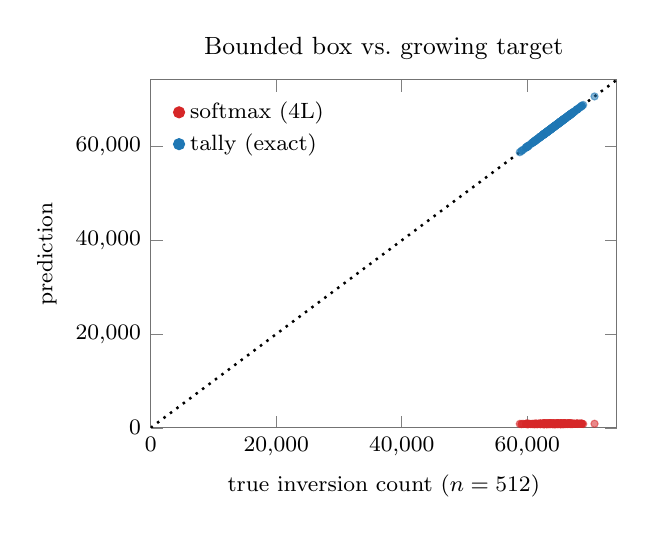
\begin{tikzpicture}
\definecolor{tabred}{RGB}{214,39,40}
\definecolor{tabblue}{RGB}{31,119,180}
\begin{axis}[
  width=7.5cm, height=6.0cm,
  xmin=0, xmax=74250.75, ymin=0, ymax=74250.75,
  xlabel={true inversion count ($n=512$)}, ylabel={prediction},
  title={Bounded box vs.\ growing target},
  tick label style={font=\footnotesize}, label style={font=\footnotesize},
  title style={font=\small,yshift=-2pt}, axis line style={black!55},
  scaled ticks=false, xtick={0,20000,40000,60000}, ytick={0,20000,40000,60000},
  legend cell align=left,
  legend style={at={(0.03,0.97)},anchor=north west,font=\footnotesize,draw=none,fill=none},
]
\addplot[black,dotted,line width=0.9pt,forget plot] coordinates {(0,0) (74250.75,74250.75)};
\addplot[only marks,mark=*,mark size=1.3pt,tabred,mark options={fill opacity=0.55,draw opacity=0.55},forget plot] coordinates {(64448.0,852.92) (64199.0,846.36) (70715.0,863.89) (65439.0,864.74) (61417.0,819.13) (65359.0,846.9) (60898.0,810.44) (67894.0,887.49) (65883.0,857.97) (66698.0,864.78) (65289.0,820.65) (65858.0,835.2) (66963.0,851.34) (66579.0,865.28) (64822.0,832.18) (61421.0,828.65) (62166.0,827.2) (65785.0,879.16) (66871.0,863.63) (65728.0,841.69) (68660.0,891.83) (63094.0,817.47) (64368.0,793.51) (64052.0,808.25) (62069.0,848.77) (66238.0,838.38) (63069.0,862.07) (59162.0,826.18) (67296.0,842.88) (62575.0,854.74) (62544.0,771.22) (63229.0,870.8) (62769.0,854.93) (63771.0,800.64) (65911.0,831.78) (65314.0,855.73) (62890.0,859.37) (68907.0,810.89) (65273.0,831.62) (65180.0,816.45) (66973.0,878.91) (64841.0,868.93) (64225.0,840.38) (66016.0,814.89) (67140.0,862.44) (64158.0,863.31) (66733.0,886.36) (66721.0,856.97) (63918.0,890.84) (63722.0,848.05) (66167.0,843.37) (64311.0,878.27) (62760.0,784.33) (65606.0,866.26) (67440.0,831.9) (63709.0,867.02) (66295.0,867.58) (64727.0,869.81) (67601.0,881.21) (65263.0,805.88) (67878.0,881.52) (64991.0,844.04) (64257.0,831.71) (59380.0,823.58) (61867.0,833.02) (65415.0,840.15) (63329.0,912.77) (65842.0,857.01) (67939.0,857.99) (63783.0,879.44) (61789.0,852.76) (65713.0,820.83) (66009.0,856.83) (66016.0,844.49) (63538.0,827.77) (66868.0,862.45) (65348.0,817.34) (66017.0,843.36) (63691.0,810.46) (66423.0,837.34) (66510.0,851.28) (64331.0,818.84) (63502.0,828.66) (66585.0,875.02) (65254.0,848.59) (64859.0,807.61) (65480.0,916.59) (66507.0,819.46) (64968.0,849.16) (62271.0,834.19) (60841.0,808.01) (66656.0,854.9) (62884.0,883.91) (66534.0,858.15) (62441.0,866.54) (63766.0,846.52) (64555.0,844.6) (68671.0,854.65) (64066.0,860.22) (64059.0,821.14) (64769.0,842.48) (65219.0,845.7) (64194.0,829.03) (66084.0,897.1) (65833.0,884.13) (64131.0,819.73) (62763.0,858.22) (64968.0,853.83) (68463.0,906.26) (63926.0,838.76) (65427.0,873.73) (68698.0,857.57) (65575.0,846.76) (65951.0,901.46) (63830.0,902.72) (62668.0,836.75) (59969.0,789.55) (65842.0,827.3) (63658.0,925.62) (62517.0,820.45) (63266.0,833.94) (63251.0,903.1) (68691.0,857.94) (65296.0,848.21) (66412.0,835.8) (65494.0,884.23) (66672.0,885.14) (65218.0,812.84) (63956.0,828.88) (67892.0,887.17) (61098.0,800.61) (66573.0,870.28) (63422.0,872.07) (66955.0,830.99) (63418.0,867.68) (62165.0,850.41) (61821.0,861.22) (63557.0,858.82) (67041.0,845.65) (63517.0,878.3) (64733.0,801.69) (64717.0,885.04) (64442.0,845.05) (64557.0,846.86) (62127.0,905.77) (62911.0,886.82) (66837.0,855.13) (65595.0,817.42) (63509.0,854.63) (66643.0,840.07) (63445.0,800.65) (61586.0,765.03) (63023.0,844.56) (66546.0,854.04) (63746.0,860.79) (62580.0,800.87) (65287.0,846.75) (64014.0,858.21) (64719.0,884.18) (66892.0,836.21) (62527.0,833.26) (68351.0,882.46) (61208.0,777.47) (63491.0,854.47) (60100.0,788.03) (67249.0,834.96) (63663.0,872.6) (65535.0,825.78) (63563.0,859.74) (64739.0,821.44) (62151.0,876.05) (67200.0,823.36) (62790.0,877.33) (62128.0,781.8) (66313.0,860.59) (64720.0,841.51) (66496.0,907.34) (63332.0,875.42) (62718.0,831.5) (59781.0,838.57) (64901.0,835.27) (63804.0,894.71) (62052.0,801.98) (65550.0,890.09) (65046.0,822.71) (64189.0,852.56) (62918.0,901.04) (63433.0,802.37) (65025.0,890.55) (64498.0,801.96) (64237.0,848.97) (65725.0,845.43) (64553.0,884.29) (65924.0,884.13) (59933.0,883.78) (64810.0,877.68) (67061.0,818.25) (66954.0,849.07) (64284.0,860.4) (64237.0,838.2) (62712.0,806.6) (62583.0,884.86) (61367.0,846.41) (66848.0,878.33) (64993.0,861.11) (63029.0,816.93) (64756.0,847.5) (66615.0,858.27) (64751.0,889.36) (64966.0,843.87) (62078.0,848.33) (65949.0,858.09) (63364.0,829.21) (66790.0,862.94) (63912.0,874.85) (63963.0,856.3) (63289.0,813.05) (60179.0,808.58) (63773.0,847.36) (65807.0,857.56) (67051.0,867.98) (65762.0,832.27) (63067.0,833.51) (65371.0,823.25) (64232.0,857.69) (60275.0,877.54) (65066.0,872.91) (63210.0,866.75) (64458.0,849.02) (63149.0,787.29) (66134.0,820.39) (66851.0,900.43) (63723.0,869.91) (65532.0,829.41) (65965.0,852.53) (62002.0,835.09) (62559.0,854.33) (64933.0,837.17) (66225.0,874.58) (61639.0,817.91) (61845.0,818.73) (62422.0,885.38) (61523.0,830.01) (67114.0,894.65) (64233.0,809.95) (65398.0,872.72) (64025.0,821.36) (64361.0,827.51) (65342.0,912.33) (64519.0,808.28) (60125.0,782.75) (63724.0,823.83) (62041.0,822.51) (63119.0,847.84) (63604.0,909.03) (64748.0,880.76) (64019.0,825.95) (68003.0,848.81) (64991.0,878.17) (63585.0,834.49) (66037.0,872.98) (63317.0,894.68) (66094.0,876.59) (66734.0,834.28) (66073.0,874.32) (65491.0,818.54) (66865.0,812.18) (61689.0,827.63) (59816.0,850.68) (61390.0,868.72) (59860.0,831.64) (65231.0,852.37) (67502.0,877.11) (63039.0,826.5) (64914.0,879.32) (63633.0,879.78) (65775.0,842.14) (64694.0,841.25) (64212.0,851.31) (62711.0,876.42) (64864.0,884.87) (62561.0,885.26) (62539.0,839.71) (61172.0,826.76) (64555.0,825.79) (65595.0,840.56) (67196.0,837.38) (68044.0,884.13) (61243.0,815.41) (59062.0,766.1) (66425.0,866.77) (65645.0,815.88) (64840.0,890.43) (64616.0,859.89) (62521.0,908.35) (66706.0,889.14) (64184.0,847.57) (62748.0,787.27) (64407.0,792.89) (66071.0,885.38) (63289.0,822.45) (65334.0,845.59) (65501.0,814.07) (60968.0,798.01) (62689.0,830.9) (62684.0,932.68) (67028.0,853.96) (65906.0,913.51) (64883.0,836.27) (65185.0,872.38) (61919.0,847.99) (61121.0,854.83) (64465.0,878.66) (63051.0,815.46) (65329.0,842.52) (64794.0,884.63) (62865.0,852.73) (61296.0,845.4) (64911.0,839.76) (64722.0,845.05) (66421.0,830.42) (63010.0,863.68) (60081.0,870.53) (65254.0,882.45) (65763.0,869.8) (63510.0,856.7) (63253.0,841.82) (62892.0,855.45) (62907.0,842.87) (66454.0,871.46) (63293.0,820.02) (63864.0,911.21) (66425.0,862.79) (60054.0,808.11) (63698.0,850.81) (62622.0,824.38) (59790.0,815.35) (58808.0,838.84) (64191.0,879.23) (64071.0,884.09) (65782.0,827.79) (64879.0,908.81) (63140.0,827.39) (64368.0,812.38) (63047.0,867.43) (66529.0,896.0) (66411.0,895.12) (65644.0,849.45) (62733.0,847.24) (65000.0,895.93) (65347.0,839.02) (64059.0,865.53) (64331.0,850.44) (65389.0,832.77) (60693.0,826.82) (65838.0,904.11) (65407.0,879.69) (64749.0,861.86) (63059.0,836.18) (68231.0,890.14) (62827.0,814.72) (62455.0,829.27) (63058.0,842.86) (65230.0,836.98) (65358.0,870.2) (62710.0,825.52) (64498.0,825.75) (66646.0,882.2) (63475.0,840.45) (65500.0,864.11) (61191.0,805.32) (63371.0,853.14) (66098.0,876.58) (65081.0,859.39) (67382.0,877.38) (65788.0,855.12) (65578.0,849.6) (66757.0,907.81) (60550.0,787.21) (65008.0,839.42) (63645.0,867.27) (60910.0,814.44) (65787.0,846.67) (65168.0,860.25)};
\addplot[only marks,mark=*,mark size=1.3pt,tabblue,mark options={fill opacity=0.55,draw opacity=0.55},forget plot] coordinates {(64448.0,64448.0) (64199.0,64199.0) (70715.0,70715.0) (65439.0,65439.0) (61417.0,61417.0) (65359.0,65359.0) (60898.0,60898.0) (67894.0,67894.0) (65883.0,65883.0) (66698.0,66698.0) (65289.0,65289.0) (65858.0,65858.0) (66963.0,66963.0) (66579.0,66579.0) (64822.0,64822.0) (61421.0,61421.0) (62166.0,62166.0) (65785.0,65785.0) (66871.0,66871.0) (65728.0,65728.0) (68660.0,68660.0) (63094.0,63094.0) (64368.0,64368.0) (64052.0,64052.0) (62069.0,62069.0) (66238.0,66238.0) (63069.0,63069.0) (59162.0,59162.0) (67296.0,67296.0) (62575.0,62575.0) (62544.0,62544.0) (63229.0,63229.0) (62769.0,62769.0) (63771.0,63771.0) (65911.0,65911.0) (65314.0,65314.0) (62890.0,62890.0) (68907.0,68907.0) (65273.0,65273.0) (65180.0,65180.0) (66973.0,66973.0) (64841.0,64841.0) (64225.0,64225.0) (66016.0,66016.0) (67140.0,67140.0) (64158.0,64158.0) (66733.0,66733.0) (66721.0,66721.0) (63918.0,63918.0) (63722.0,63722.0) (66167.0,66167.0) (64311.0,64311.0) (62760.0,62760.0) (65606.0,65606.0) (67440.0,67440.0) (63709.0,63709.0) (66295.0,66295.0) (64727.0,64727.0) (67601.0,67601.0) (65263.0,65263.0) (67878.0,67878.0) (64991.0,64991.0) (64257.0,64257.0) (59380.0,59380.0) (61867.0,61867.0) (65415.0,65415.0) (63329.0,63329.0) (65842.0,65842.0) (67939.0,67939.0) (63783.0,63783.0) (61789.0,61789.0) (65713.0,65713.0) (66009.0,66009.0) (66016.0,66016.0) (63538.0,63538.0) (66868.0,66868.0) (65348.0,65348.0) (66017.0,66017.0) (63691.0,63691.0) (66423.0,66423.0) (66510.0,66510.0) (64331.0,64331.0) (63502.0,63502.0) (66585.0,66585.0) (65254.0,65254.0) (64859.0,64859.0) (65480.0,65480.0) (66507.0,66507.0) (64968.0,64968.0) (62271.0,62271.0) (60841.0,60841.0) (66656.0,66656.0) (62884.0,62884.0) (66534.0,66534.0) (62441.0,62441.0) (63766.0,63766.0) (64555.0,64555.0) (68671.0,68671.0) (64066.0,64066.0) (64059.0,64059.0) (64769.0,64769.0) (65219.0,65219.0) (64194.0,64194.0) (66084.0,66084.0) (65833.0,65833.0) (64131.0,64131.0) (62763.0,62763.0) (64968.0,64968.0) (68463.0,68463.0) (63926.0,63926.0) (65427.0,65427.0) (68698.0,68698.0) (65575.0,65575.0) (65951.0,65951.0) (63830.0,63830.0) (62668.0,62668.0) (59969.0,59969.0) (65842.0,65842.0) (63658.0,63658.0) (62517.0,62517.0) (63266.0,63266.0) (63251.0,63251.0) (68691.0,68691.0) (65296.0,65296.0) (66412.0,66412.0) (65494.0,65494.0) (66672.0,66672.0) (65218.0,65218.0) (63956.0,63956.0) (67892.0,67892.0) (61098.0,61098.0) (66573.0,66573.0) (63422.0,63422.0) (66955.0,66955.0) (63418.0,63418.0) (62165.0,62165.0) (61821.0,61821.0) (63557.0,63557.0) (67041.0,67041.0) (63517.0,63517.0) (64733.0,64733.0) (64717.0,64717.0) (64442.0,64442.0) (64557.0,64557.0) (62127.0,62127.0) (62911.0,62911.0) (66837.0,66837.0) (65595.0,65595.0) (63509.0,63509.0) (66643.0,66643.0) (63445.0,63445.0) (61586.0,61586.0) (63023.0,63023.0) (66546.0,66546.0) (63746.0,63746.0) (62580.0,62580.0) (65287.0,65287.0) (64014.0,64014.0) (64719.0,64719.0) (66892.0,66892.0) (62527.0,62527.0) (68351.0,68351.0) (61208.0,61208.0) (63491.0,63491.0) (60100.0,60100.0) (67249.0,67249.0) (63663.0,63663.0) (65535.0,65535.0) (63563.0,63563.0) (64739.0,64739.0) (62151.0,62151.0) (67200.0,67200.0) (62790.0,62790.0) (62128.0,62128.0) (66313.0,66313.0) (64720.0,64720.0) (66496.0,66496.0) (63332.0,63332.0) (62718.0,62718.0) (59781.0,59781.0) (64901.0,64901.0) (63804.0,63804.0) (62052.0,62052.0) (65550.0,65550.0) (65046.0,65046.0) (64189.0,64189.0) (62918.0,62918.0) (63433.0,63433.0) (65025.0,65025.0) (64498.0,64498.0) (64237.0,64237.0) (65725.0,65725.0) (64553.0,64553.0) (65924.0,65924.0) (59933.0,59933.0) (64810.0,64810.0) (67061.0,67061.0) (66954.0,66954.0) (64284.0,64284.0) (64237.0,64237.0) (62712.0,62712.0) (62583.0,62583.0) (61367.0,61367.0) (66848.0,66848.0) (64993.0,64993.0) (63029.0,63029.0) (64756.0,64756.0) (66615.0,66615.0) (64751.0,64751.0) (64966.0,64966.0) (62078.0,62078.0) (65949.0,65949.0) (63364.0,63364.0) (66790.0,66790.0) (63912.0,63912.0) (63963.0,63963.0) (63289.0,63289.0) (60179.0,60179.0) (63773.0,63773.0) (65807.0,65807.0) (67051.0,67051.0) (65762.0,65762.0) (63067.0,63067.0) (65371.0,65371.0) (64232.0,64232.0) (60275.0,60275.0) (65066.0,65066.0) (63210.0,63210.0) (64458.0,64458.0) (63149.0,63149.0) (66134.0,66134.0) (66851.0,66851.0) (63723.0,63723.0) (65532.0,65532.0) (65965.0,65965.0) (62002.0,62002.0) (62559.0,62559.0) (64933.0,64933.0) (66225.0,66225.0) (61639.0,61639.0) (61845.0,61845.0) (62422.0,62422.0) (61523.0,61523.0) (67114.0,67114.0) (64233.0,64233.0) (65398.0,65398.0) (64025.0,64025.0) (64361.0,64361.0) (65342.0,65342.0) (64519.0,64519.0) (60125.0,60125.0) (63724.0,63724.0) (62041.0,62041.0) (63119.0,63119.0) (63604.0,63604.0) (64748.0,64748.0) (64019.0,64019.0) (68003.0,68003.0) (64991.0,64991.0) (63585.0,63585.0) (66037.0,66037.0) (63317.0,63317.0) (66094.0,66094.0) (66734.0,66734.0) (66073.0,66073.0) (65491.0,65491.0) (66865.0,66865.0) (61689.0,61689.0) (59816.0,59816.0) (61390.0,61390.0) (59860.0,59860.0) (65231.0,65231.0) (67502.0,67502.0) (63039.0,63039.0) (64914.0,64914.0) (63633.0,63633.0) (65775.0,65775.0) (64694.0,64694.0) (64212.0,64212.0) (62711.0,62711.0) (64864.0,64864.0) (62561.0,62561.0) (62539.0,62539.0) (61172.0,61172.0) (64555.0,64555.0) (65595.0,65595.0) (67196.0,67196.0) (68044.0,68044.0) (61243.0,61243.0) (59062.0,59062.0) (66425.0,66425.0) (65645.0,65645.0) (64840.0,64840.0) (64616.0,64616.0) (62521.0,62521.0) (66706.0,66706.0) (64184.0,64184.0) (62748.0,62748.0) (64407.0,64407.0) (66071.0,66071.0) (63289.0,63289.0) (65334.0,65334.0) (65501.0,65501.0) (60968.0,60968.0) (62689.0,62689.0) (62684.0,62684.0) (67028.0,67028.0) (65906.0,65906.0) (64883.0,64883.0) (65185.0,65185.0) (61919.0,61919.0) (61121.0,61121.0) (64465.0,64465.0) (63051.0,63051.0) (65329.0,65329.0) (64794.0,64794.0) (62865.0,62865.0) (61296.0,61296.0) (64911.0,64911.0) (64722.0,64722.0) (66421.0,66421.0) (63010.0,63010.0) (60081.0,60081.0) (65254.0,65254.0) (65763.0,65763.0) (63510.0,63510.0) (63253.0,63253.0) (62892.0,62892.0) (62907.0,62907.0) (66454.0,66454.0) (63293.0,63293.0) (63864.0,63864.0) (66425.0,66425.0) (60054.0,60054.0) (63698.0,63698.0) (62622.0,62622.0) (59790.0,59790.0) (58808.0,58808.0) (64191.0,64191.0) (64071.0,64071.0) (65782.0,65782.0) (64879.0,64879.0) (63140.0,63140.0) (64368.0,64368.0) (63047.0,63047.0) (66529.0,66529.0) (66411.0,66411.0) (65644.0,65644.0) (62733.0,62733.0) (65000.0,65000.0) (65347.0,65347.0) (64059.0,64059.0) (64331.0,64331.0) (65389.0,65389.0) (60693.0,60693.0) (65838.0,65838.0) (65407.0,65407.0) (64749.0,64749.0) (63059.0,63059.0) (68231.0,68231.0) (62827.0,62827.0) (62455.0,62455.0) (63058.0,63058.0) (65230.0,65230.0) (65358.0,65358.0) (62710.0,62710.0) (64498.0,64498.0) (66646.0,66646.0) (63475.0,63475.0) (65500.0,65500.0) (61191.0,61191.0) (63371.0,63371.0) (66098.0,66098.0) (65081.0,65081.0) (67382.0,67382.0) (65788.0,65788.0) (65578.0,65578.0) (66757.0,66757.0) (60550.0,60550.0) (65008.0,65008.0) (63645.0,63645.0) (60910.0,60910.0) (65787.0,65787.0) (65168.0,65168.0)};
\addlegendimage{only marks,mark=*,tabred,mark size=2pt}\addlegendentry{softmax (4L)}
\addlegendimage{only marks,mark=*,tabblue,mark size=2pt}\addlegendentry{tally (exact)}
\end{axis}
\end{tikzpicture}

\caption{The box, photographed. Predictions against true inversion count
for length-512 lists. The dashed diagonal is where a correct model would
sit. The tally head with hand-set weights sits on it. The trained softmax
model does not: every one of its predictions falls inside a band about
$166$ wide, while the true counts run past $65{,}000$. This is
Lemma~\ref{lem:bounded} made visible. The model is not making a small
mistake, it is answering from a range that no longer contains the
answer.}
\label{fig:scatter}
\end{figure}

The obvious objection is whether this is a real architectural wall or just
a model failing on new data, which would be a fake collapse. To rule that
out, we ensured the baseline models were fully trained under a rigorous
training budget, and we scaled up by roughly $7\times$ using Qwen models.
It does not move the wall. Section~\ref{sec:results} reports both
controls.

\begin{figure}[htbp]
\centering
% Drawn for this paper. Left: the convex hull of four value vectors, with several
% admissible head outputs inside it; the cage idea is Richter and Wattenhofer's,
% the drawing is ours. Right: the readout's box against the counts it must reach,
% plotted from the formulas, not from any measurement.
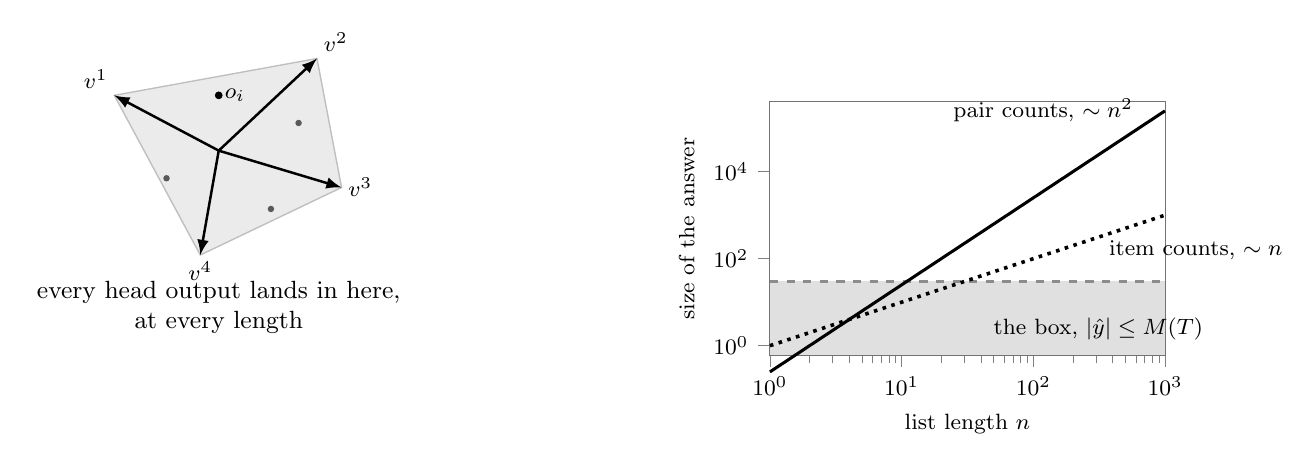
\begin{tikzpicture}
\begin{scope}[scale=0.78]
  \coordinate (O)  at (0,0);
  \coordinate (V1) at (-1.7, 0.9);
  \coordinate (V2) at ( 1.6, 1.5);
  \coordinate (V3) at ( 2.0,-0.6);
  \coordinate (V4) at (-0.3,-1.7);
  \fill[black!8,draw=black!25,line width=0.5pt] (V1) -- (V2) -- (V3) -- (V4) -- cycle;
  \foreach \v/\lab/\pos in {V1/{v^{1}}/{above left}, V2/{v^{2}}/{above right},
                            V3/{v^{3}}/{right}, V4/{v^{4}}/{below}}
    \draw[-latex,line width=0.9pt] (O) -- (\v) node[\pos,font=\footnotesize,inner sep=2pt] {$\lab$};
  \fill[black!65] (-0.85,-0.45) circle (1.5pt);
  \fill[black!65] ( 1.30, 0.45) circle (1.5pt);
  \fill[black!65] ( 0.85,-0.95) circle (1.5pt);
  \fill (0.00,0.90) circle (1.8pt) node[right,font=\footnotesize,inner sep=2pt] {$o_i$};
  \node[font=\small,align=center] at (0,-2.55) {every head output lands in here,\\at every length};
\end{scope}
\begin{scope}[xshift=7.0cm,yshift=-2.6cm]
\begin{axis}[
  width=6.6cm, height=4.8cm,
  xmode=log, ymode=log, log basis x=10,
  domain=1:1000, samples=80,
  xmin=1, xmax=1000, ymin=0.6, ymax=4e5,
  ytickten={0,2,4},
  xlabel={list length $n$}, ylabel={size of the answer},
  tick label style={font=\footnotesize}, label style={font=\footnotesize},
  tick align=outside, tick pos=left,
  axis line style={black!55},
  clip=false,
]
% the box the readout can reach: fixed by the weights, not by n
\fill[black!12] (axis cs:1,0.6) rectangle (axis cs:1000,30);
\draw[black!45,dashed,line width=0.8pt] (axis cs:1,30) -- (axis cs:1000,30);
\node[anchor=west,font=\footnotesize,inner sep=2pt] at (axis cs:45,2.4)
  {the box, $|\hat{y}|\le M(T)$};
\addplot[black,line width=1.1pt] {x*x/4};
  \node[anchor=south east,font=\footnotesize,inner sep=1.5pt,yshift=1pt]
    at (axis cs:620,96100) {pair counts, $\sim n^{2}$};
\addplot[black,dotted,line width=1.3pt] {x};
  \node[anchor=north west,font=\footnotesize,inner sep=1.5pt,xshift=1pt]
    at (axis cs:330,330) {item counts, $\sim n$};
\end{axis}
\end{scope}
\end{tikzpicture}

\caption{The probability cage, and what each aggregator does as $n$ grows.
Left: every softmax head output is a convex combination of its value
vectors, so it can never leave the convex hull they span, whatever the
weights are. Right: the scaling forms themselves, plotted from their
formulas rather than measured. An unnormalized sum of $n$ comparable terms
grows like $\sqrt{n}$, a normalized readout stays flat, and an average sinks
like $1/\sqrt{n}$. The geometry on the left is the one
\citet{richter2020cage} name the probability cage.}
\label{fig:aggregators}
\end{figure}

\subsection{The Bounded Readout Lemma}

\begin{lemma}[Bounded Readout]
\label{lem:bounded}
For every $T \in \mathcal{T}$,
\begin{equation}
\exists\, M(T) < \infty \quad\text{such that}\quad |\hat{y}(x)| \leq M(T)
\qquad\text{for every input } x .
\label{eq:bounded}
\end{equation}
\end{lemma}

Once you know a particular Transformer $T$, there is a finite maximum-sized
box that contains every one of its one-shot numerical outputs, regardless
of how long the list becomes. The box might be huge, but the theorem does
not care.

\begin{remark}[{Why $[-M(T), M(T)]$ and not $[0, M(T)]$}]
\label{rem:whysymmetric}
Because the model's \emph{prediction} can be negative, even though the
true count cannot. Its final readout is usually a linear layer,
$\hat{y} = w^{\top}h + b$, and a linear layer can produce $-8$, $-0.4$,
$2.7$, $100$, and so on. So the proof safely says $|\hat{y}| \leq M(T)$,
which means $-M(T) \leq \hat{y} \leq M(T)$. If we forced the model to
output only nonnegative numbers, for example with a ReLU at the end, then
we could use $[0, M(T)]$. That would give the model \emph{fewer}
answer slots, so the impossibility would only be stronger.
\end{remark}

\subsection{Why attention is bounded}
\label{sec:why-bounded}

Suppose every value vector has size at most $B_V$, so that
$\|v_j\| \leq B_V$. Attention outputs $o_i = \sum_j w_{ij} v_j$, and by the
triangle inequality,
\begin{equation}
\|o_i\| \;\leq\; \sum_j w_{ij}\,\|v_j\|
        \;\leq\; \left(\sum_j w_{ij}\right) B_V
        \;\leq\; B_V .
\label{eq:attn-bound}
\end{equation}
So the attention output cannot be larger than the largest value it mixed.
This is derived from the triangle inequality, $|x+y| \leq |x| + |y|$. It is
the same idea for vectors as for numbers, except that here it is in the
$L^2$ norm.

Notice what does \emph{not} appear in that bound:
\begin{itemize}
\item the number of tokens $n$;
\item the number of matching tokens;
\item the sharpness of attention;
\item the temperature;
\item the raw attention scores.
\end{itemize}

That is why ``make attention sharper'' is not a theoretical escape. It
changes \emph{which} values receive weight, but the weights still total
one.

\begin{proof}[Proof of Lemma~\ref{lem:bounded}]
We show that for any standard Transformer with a single-pass readout, the
final prediction $\hat y$ is mathematically trapped within a fixed-size
box, $|\hat y| \leq M(T)$, whose size is determined entirely by the
network's weights and does not depend on the length $n$ of the input list.

\begin{enumerate}
\item \textbf{LayerNorm re-bounds the state.} At every layer, LayerNorm
  stretches the vector to a fixed length ($\sqrt{d}$) and applies a fixed
  scale and shift. Therefore, after any LayerNorm, the state has a
  strictly bounded size, regardless of how large the numbers were when
  they entered.

\item \textbf{Attention is a convex average (the crux).} An attention head
  outputs $\sum_j w_{ij} v_j$ with $w_{ij} \geq 0$ and
  $\sum_j w_{ij} \leq 1$. By Eq.~\eqref{eq:attn-bound}, the output length
  can never exceed $\max_j \|v_j\|$. Crucially, the input length $n$ and
  the raw attention scores never appear in this bound. Therefore
  temperature scaling, sparsemax, and $\alpha$-entmax cannot solve
  counting, because they only redistribute the weights; they never enlarge
  the average.

\item \textbf{Finitely many layers.} The network has a fixed depth of $L$
  blocks. Adding together $L$ bounded increments means the final state
  remains inside a fixed-size ball.

\item \textbf{Readout.} A fixed, continuous readout head applied to that
  bounded ball produces a strictly bounded final output, $M(T)$.
  \qedhere
\end{enumerate}
\end{proof}

\subsection{Consequence (a): the error must eventually become huge}
\label{sec:conseq-a}

A counting problem becomes harder as the input gets longer. For example,
the number of inverted pairs in a list can grow roughly like $n^2$. But
the Transformer's output is trapped inside a fixed range, from $-M(T)$ to
$M(T)$, no matter how long the input becomes.

Consider a list made of a block of $1$s followed by a block of $0$s, for
example $1\,1\,1\,1\,1\,0\,0\,0\,0\,0$. Every $1$ comes before every $0$,
so with $n/2$ ones and $n/2$ zeros the number of inversions grows roughly
like $n^2/4$. The model's prediction must remain inside $[-M(T), M(T)]$
while the correct answer keeps increasing. Therefore, for sufficiently
long lists, the model's error must grow without limit.

This also means the model cannot get even close. If the output box goes up
to $100$ but the true answer is $60{,}000$, it physically cannot reach the
answer, and the failure is precision-free. No matter how many floating-point
or decimal places the model has, no precision will help a number reach a
value it is trapped below. The problem is not numerical precision. The
correct answer eventually lies completely outside the model's output
range.

We define $\max_x |\hat{y}(x) - \Inv(x)|$ as the largest error there is,
which we can also call the worst-case error.

Saying the error grows without limit is true, but we can say exactly how
big it gets. Take that
same two-block list, $n/2$ ones followed by $n/2$ zeros. Every one sits
before every zero, so its inversion count is exactly $\lfloor n^2/4
\rfloor$, and we already know the prediction cannot be further than $M(T)$
from zero. The gap between the two is then at least
\[
  \max_x |\hat{y}(x) - \Inv(x)| \;\ge\; \lfloor n^2/4 \rfloor - M(T).
\]
So the error does not just grow, it grows quadratically, and it does so
past a critical length that depends only on the weights.

One list is enough to prove that, which is not what we expected when we
first tried it; our first attempt compared two lists and got a bound half
as strong. Appendix~\ref{app:proofs} keeps that two-list version anyway,
because it survives on weaker assumptions.



\noindent Worst-case error means the largest error over all lists of a
given length, not the average one. A model that is off by $2$ on one list,
by $1$ on another and by $6$ on a third has worst-case error $6$. What we
prove is a floor under that quantity:
\begin{equation}
\max_x \big|\hat{y}(x) - \Inv(x)\big| \;\geq\; \lfloor n^2/4 \rfloor - M(T),
\label{eq:worstcase}
\end{equation}
where $\hat{y}(x)$ is the model prediction and $\Inv(x)$ is the true
count. The step-by-step derivation is in Appendix~\ref{app:proofs},
together with the weaker two-list bound and the reason we keep it on file.

\subsection{Consequence (b): exact counting eventually becomes impossible}
\label{sec:conseq-b}

Suppose we interpret the model's output by rounding it to the nearest
whole number. Because the output is restricted to a fixed interval, the
model can produce only a limited number of distinct integer answers.
However, as the input length increases, the number of possible correct
counts keeps growing. Eventually there are more possible correct answers
than available model outputs, and when the model is forced to squeeze all
of them together, it runs out of places to differentiate them.

By the pigeonhole principle, at least two inputs with different correct
counts must receive the same prediction. Thus, for every fixed model $T$,
there is a sufficiently large input length $n$ such that the model cannot
correctly return the integer inversion count for every possible list of
length $n$, regardless of how its parameters are chosen.

\begin{example}[The pigeonhole, made concrete]
Suppose the output bound is $[-M(T), M(T)] = [-3, 3]$. After rounding, the
possible integer answers are $-3, -2, -1, 0, 1, 2, 3$, which is only seven
slots.
Now imagine an input length at which inversion counts range from $0$ to
$9$. Ten true answers cannot fit into seven slots without at least two
sharing one.
\end{example}

%=======================================================================
\subsection{What is not blocked: the Boolean twin}
\label{sec:dichotomy}

The barrier is a statement about \emph{extensive} quantities, answers that
grow with the list. A yes-or-no question about the same list is
\emph{intensive}: however long the list gets, the answer stays $0$ or $1$
and fits inside the finite box with room to spare. Ask the list
$4, 2, 3, 1$ two questions. How many inversions does it have? The answer
is $5$ here and can be $50{,}000$ on a longer list, and this is what
Theorem~\ref{thm:barrier} blocks. Is there at least one inversion? That
answer is never anything but yes or no. Formally, for a counting function
$F$ we define its detection twin as
\begin{equation}
\hat{F}(x) \;=\; \mathbf{1}\big[F(x) > 0\big],
\label{eq:detect}
\end{equation}
so for inversions $\mathrm{Detect}(x) = \mathbf{1}[\Inv(x) > 0]$: the list
$1,2,3$ has $\Inv = 0$ and $\mathrm{Detect} = 0$, while $3,1,2$ has
$\Inv = 2$ and $\mathrm{Detect} = 1$. The model is not blind. It can
genuinely detect, and what it cannot do with bounded resources is output a
growing total. Section~\ref{sec:twincontrol} turns this contrast into the
paper's sharpest control, running Detect and Count through the same
readout on identical inputs.

\subsection{The complete list of ways out}
\label{sec:escapes-list}

A barrier on its own is only a complaint about softmax. What makes this a
characterization is being able to say what the alternatives are without
leaving any out, and the reason we can is structural rather than clever. The
five conditions in Section~\ref{sec:classT} are not extra requirements
bolted onto the class. They \emph{are} the class. So failing one of them is
exactly what it means to be outside it, and Theorem~\ref{thm:barrier} rules
out everything inside. A model that does emit a growing count therefore has
to fail one of the five, and listing the conditions lists the ways out with
nothing left over.

\begin{table}[htbp]
\centering
\caption{The ways out, one per condition. The last column is the one that
matters in practice: for a fixed single-pass numeric readout, three of the
five are already closed before anything gets designed.}
\label{tab:escapes}
\small
\begin{tabular}{@{}p{2.5cm}p{3.6cm}p{3.3cm}p{3.6cm}@{}}
\toprule
\textbf{Condition} & \textbf{The way out} & \textbf{Where it is used} & \textbf{Open to a one-pass readout?} \\
\midrule
Bounded input features & an input feature that grows with $n$ & graph networks feeding a node its degree & No. A finite alphabet bounds the embeddings automatically \\
\addlinespace
Bounded positions & positions entered as a raw growing index & any model handed the index or the length itself & No, not for rotary, sinusoidal or ALiBi encodings \\
\addlinespace
Sub-convex mixing & drop the requirement that weights total at most one & sigmoid attention, ReLU attention, sum-pooling & Yes. This is half of the fix \\
\addlinespace
Fixed depth & depth that grows with the input & no deployed model & No. Depth is fixed before the input arrives \\
\addlinespace
Fixed single-pass readout & emit the answer over several tokens & chain of thought, or a tool call where a database does the adding & No. A readout that emits tokens is a generator \\
\addlinespace
 & or rescale by $n$ outside the network & the fraction readout & Yes, at a price we measure \\
\bottomrule
\end{tabular}
\end{table}

Three of the five are shut before you start. A language model over a finite
alphabet has bounded embeddings whether it wants them or not, deployed
models fix their depth in advance, and a readout that writes tokens has become a generator. That leaves two, and one of them is
rescaling by $n$ outside the model, which we run as a baseline and which
trades the range problem for a resolution problem. So the additive path is
not one option among many. It is what is left once the others are counted
off. The list belongs here, not in a limitations paragraph.

It also makes the theorem refutable in the ordinary way. Show us a network
inside the class that emits a growing count and the theorem is finished. We name that refutation, rule it out, and then run every near miss we could
build, which is sharper attention, $\log n$ scaling, more depth and width,
the fraction readout, and the same head with its denominator put back. They
all land where the theorem says they have to.

%=======================================================================
\section{The Tally Head}
\label{sec:tally}
%=======================================================================

\begin{theorem}[One-Head Universality]
\label{thm:universal}
For every fixed item rule $\varphi$ and every fixed pair rule $P$ over a
finite alphabet, there exists a setting of a single additive tally head's
query and key weights that computes the resulting count
$F_{\varphi,P}$ exactly, at every length.
\end{theorem}

In other words, for every fixed counting rule there exists a setting of the
tally head's query/key weights that counts that rule exactly: one weight
setting for inversions, a different weight setting for duplicates, and so
on.

Theorem~\ref{thm:barrier} says that normal attention fails because
$o_i = \sum_j w_{ij} v_j$ with $\sum_j w_{ij} = 1$ makes an
\emph{average}. The tally head keeps the useful part, which is the pairwise
comparison, but removes the denominator and sets it to one, so the
result is an unnormalized \emph{sum} rather than a weighted average.

\subsection{Definition}

\begin{definition}[Tally head]
\label{def:tally}
\begin{equation}
y_{\text{tally}} \;=\; \sum_i \sum_{j<i} \clampf\big(\ell_{ij},\, 0,\, 1\big),
\label{eq:tally}
\end{equation}
where $\ell_{ij}$ is the raw comparison score after multiplication, also
known as the logit; the clamp gate turns it into a vote; the sum runs over
every pair obeying $j < i$; and $y_{\text{tally}}$ is the final count.
\end{definition}

The clamp gate is
\begin{equation}
\clampf(t, 0, 1) \;=\;
\begin{cases}
0, & t \leq 0,\\
t, & 0 < t < 1,\\
1, & t \geq 1.
\end{cases}
\label{eq:clamp}
\end{equation}

The pipeline is: pair comparisons $\rightarrow$ clamp into $0/1$ votes
$\rightarrow$ sum votes $\rightarrow$ scalar output.

\begin{remark}[Notation]
\label{rem:phi-collision}
An earlier version of this construction wrote the clamp gate as $\phi$, and also wrote the
one-item rule as $\varphi$. To keep the two apart, this paper writes the
clamp explicitly as $\clampf(\cdot, 0, 1)$ throughout and reserves
$\varphi$ for the item rule of Eq.~\eqref{eq:class}.
\end{remark}

\subsection{The hand-built construction for inversion counting}
\label{sec:handbuilt}

We know that $\ell_{ij}$ is the dot product of the query vector of $i$ and
the key vector of $j$. We now want $\ell_{ij}$ to equal $a_j - a_i$,
because an inversion happens exactly when $a_j > a_i$. The methodology is
to work backwards from the score we want, $\ell_{ij} = a_j - a_i$.

We call this construction \emph{hand-built} because we choose the vectors
and weights using pure linear algebra: there is no training data, no
gradient descent, and no backpropagation.

\paragraph{Step 1: factor the difference.}
\[
a_j - a_i \;=\; (a_j,\, 1) \cdot (1,\, -a_i).
\]
Therefore choose
\begin{equation}
q_i = (1,\, -a_i), \qquad k_j = (a_j,\, 1).
\label{eq:qk-inv}
\end{equation}

\paragraph{Step 2: map everything into coordinate form.}
Treating the query and key as two-coordinate vectors and multiplying the
corresponding coordinates,
\[
q_i \cdot k_j \;=\; 1 \times a_j + (-a_i) \times 1 \;=\; a_j - a_i .
\]

\begin{example}[Two pairs from $(4,2,3,1)$]
\label{ex:qk}
Take earlier value $4$ and later value $2$:
\[
q_i = (1, -2), \qquad k_j = (4, 1), \qquad
\ell_{ij} = (1,-2)\cdot(4,1) = 4 - 2 = 2 .
\]
Positive, so it is an inversion. Now take earlier value $2$ and later
value $3$: $\ell_{ij} = 2 - 3 = -1$. Negative, so it is not an inversion.
\end{example}

\paragraph{Step 3: the clamp turns the score into the vote.}

For integer-valued items the gap $a_j - a_i$ is itself an integer, so it is
at least $1$ whenever the pair is an inversion and at most $0$ whenever it
is not. The clamp sends everything at or above $1$ to exactly $1$ and
everything at or below $0$ to exactly $0$. There is nothing in between for
it to land on, so the gate is exact and not an approximation.

\noindent Therefore
\begin{equation}
\clampf(a_j - a_i,\, 0,\, 1) \;=\; \mathbf{1}[a_j > a_i].
\label{eq:key-equality}
\end{equation}
This is the key equality: the tally head's gate is now exactly the same as
the inversion indicator in the mathematical definition.

\paragraph{Step 4: substitute.}
Since $\ell_{ij} = a_j - a_i$ and, for integer-valued items,
Eq.~\eqref{eq:key-equality} holds, substituting into
Eq.~\eqref{eq:tally} gives
\[
y_{\text{tally}} \;=\; \sum_i \sum_{j<i} \mathbf{1}[a_j > a_i]
\;=\; \Inv(a),
\]
which is exactly Eq.~\eqref{eq:inv}. Hence the tally head returns the
exact inversion count for any list length. \qed

\subsection{What happens when the numbers are not whole}
\label{sec:gamma}

The construction works on integers because integers are at least one apart,
so the clamp always lands cleanly on $0$ or $1$. Real numbers are not that
tidy, and we would rather write down what happens than leave it as a hidden assumption. Say the values are real and we scale the comparison by some
$\gamma$ larger than zero, so the head computes
\[
  y_{\gamma}(x) \;=\; \sum_{i} \sum_{j < i} \phi\!\left( (a_j - a_i)/\gamma \right).
\]
Call a pair a near-tie when the earlier number really is bigger than the
later one, but by less than $\gamma$, and write $A_{\gamma}(x)$ for how many
near-ties the list contains. Then
\[
  0 \;\le\; \Inv(x) - y_{\gamma}(x) \;\le\; A_{\gamma}(x).
\]

The reason is that a pair can only do one of three things. If the earlier
number is bigger by $\gamma$ or more, the scaled difference is at least $1$,
the clamp gives exactly $1$, and that is the right answer. If the earlier
number is not bigger at all, the difference is zero or negative, the clamp
gives $0$, and that is also right, since inversions use a strict inequality
and ties are not supposed to count. That leaves the near-ties, where the
clamp returns something between $0$ and $1$ while the truth is $1$. Each
one costs at most one, and each one costs in the same direction. So the head
can undercount and can never overcount, which means the number it returns is a lower bound on the true count, wrong in one direction only.

Two things follow. The size of the error depends on how crowded the values
are and not on how long the list is, so on any input whose numbers are
spread out relative to $\gamma$ the count stays exact at every length, which
is the thing the barrier says no normalized readout can manage. And since
$A_{\gamma}$ falls to zero as soon as $\gamma$ drops below the smallest
positive gap in the list, the construction is exact on every input if one is free to choose $\gamma$. The only reason to fix it in advance is
numerical, since the comparison gets scaled by $1/\gamma$ and shrinking
$\gamma$ trades accuracy against dynamic range. That is a floating-point
tradeoff and the inequality above bounds it. It is not the range wall from
Theorem~\ref{thm:barrier}, which no choice of constant can move.

\subsection{Why we construct rather than train}
\label{sec:why-construct}

At this point the head can only count inversions, but we want it to
generalize across all questions, which is what
Theorem~\ref{thm:universal} does. We design the weights by mathematical
construction instead of training, because construction answers the key
question: \emph{can this architecture do that at all?} Our hand-built
construction proves that the architecture has the representational ability
to count exactly, so a failure cannot be blamed on bad initialization, bad
training data, or a poor optimizer.

Training answers a different question: \emph{can gradient descent discover
this at all?} That is an experiment, not a theorem. Later
(Section~\ref{sec:robustness}) we found that dead clamp gates can prevent
learning entirely, that active-region initialization repairs that problem,
and that several pairwise rules together are not reliably learned across
seeds. Training a model until it fits a pattern can be useful, but it does not
prove exactness and it does not guarantee success.

\subsection{Proof sketch of Theorem~\ref{thm:universal}}
\label{sec:proof-sketch}

Both halves rest on one lookup-table fact. Over a finite alphabet, any
fixed pair rule $P$ is a finite table of $0$s and $1$s. Give each value $a$
the one-hot key $k(a) = e_a$, and give each value $b$ a query $q(b)$ whose
$a$-th entry is $P(a, b)$. The dot product then reads the table directly,
$q(b) \cdot k(a) = P(a, b)$, so the score for a pair is already the $0$ or
$1$ vote we want, the clamp leaves it untouched, and the un-normalized sum
counts exactly the pairs the rule accepts. The item-wise half is the same
idea one level down: a single vector $u$ holding the truth table of
$\varphi$ gives $u \cdot e_{a_i} = \varphi(a_i)$. The full proofs, with a
worked ``pairs summing to $2$'' example and a remark on what is and is not
being claimed, are in Appendix~\ref{app:proofs}.

\subsection{The complete universal tally head}
\label{sec:universal-head}
\label{sec:complete}

Combining the two channels:
\begin{equation}
y(x) \;=\;
\underbrace{\sum_i \clampf\big(\langle u, f(a_i)\rangle, 0, 1\big)}_{\text{items satisfying } \varphi}
\;+\;
\underbrace{\sum_i \sum_{j<i} \clampf\big(\langle W_Q f(a_i), W_K f(a_j)\rangle, 0, 1\big)}_{\text{pairs satisfying } P}.
\label{eq:complete}
\end{equation}
Because the hand-built scores are already $0$ or $1$, the clamps do
nothing harmful. Therefore
\[
y(x) \;=\; \sum_i \varphi(a_i) + \sum_i\sum_{j<i} P(a_j, a_i) \;=\; F_{\varphi,P}(x),
\]
which completes Theorem~\ref{thm:universal}: for every fixed item rule
$\varphi$ and pair rule $P$ over a finite alphabet, one additive tally
head can compute the resulting count exactly, at every length. \qed

\begin{corollary}[Zero versus one]
\label{cor:zeroone}
From Theorem~\ref{thm:barrier}: a standard fixed-depth, normalized
(including softmax), one-shot Transformer has zero additive heads, and it
cannot emit any non-trivial count that grows with list length. From
Theorem~\ref{thm:universal}: adding one unnormalized tally head with
constructed weights lets it exactly compute any fixed item-wise or
pairwise count in our class. The crux is therefore that \emph{zero
additive heads suffice for none of these unbounded counting tasks, and one
additive head suffices for all of them.}
\end{corollary}

\subsection{How the head is wired in}
\label{sec:wiring}

The head runs beside the normal model rather than inside it. Each yes/no
question becomes a clean $0/1$ through the clamp gate, and the votes are
summed on a private wire that bypasses the normalized path and can never be
squashed on the way to the readout. We place it in two positions: layer $0$
for pair counting, which handicaps it deliberately and asks whether it can
count with no help from the trunk, and the mid-stack layer $14$, where it
has to answer questions posed in plain English.

The hand-built version is just algebra. Each item gets the features
$(1, a, a^2)$, so the query and key comparison can act as a small formula;
for inversions that formula subtracts the later number from the earlier
one, the clamp snaps the integer difference to $1$ or $0$, and the private
wire adds the votes up. Nothing is trained at all. And the same wiring
covers every other rule, for the reason given in
Section~\ref{sec:universal-head}: a yes/no rule over a finite alphabet is
just a table of $1$s and $0$s, and a query and key product reproduces any
such table exactly. So we do not need a new tool for every question, and we
never touch the existing architecture.

There is an obvious worry about bolting anything onto a model that already
works, which is that it might quietly break something it used to do right.
For this head that can be settled by looking at the wiring instead of by
running benchmarks, and we prefer the argument, because a benchmark can only
fail to find damage while the argument rules it out.

Keep the trunk frozen. Let the head read hidden states without writing
anything back into the residual stream, and give its answer its own output
coordinate that the original outputs never look at. Then every hidden state
in the new model equals the one in the old model. That follows by induction
over the layers: layer $\ell+1$ depends on the residual stream at layer
$\ell$ and on nothing else, and the head never puts anything into that
stream, so if the streams match at one layer they match at the next. They
match at the input, so they match all the way through. The final states are
therefore the same, and every original output is the same fixed function of
the same final state. Not close to the same. Identical, bit for bit, since
the original computation was never touched at all. Turning the head off by
setting its output coefficient to zero gives back the original model
exactly.

There are two things this does not cover. It is a statement about the
computation and not about a deployment, so a router that decides when to
consult the head is a separate piece and can certainly get things wrong.
And it assumes the trunk stays frozen. Train the head jointly with the
trunk and it is a different object, and none of this applies. Every
experiment in this paper keeps the trunk frozen.

%=======================================================================
\section{Experiments}
\label{sec:setup}\label{sec:results}
%=======================================================================

We test the two theorems on three testbeds, ordered from the wild to the
controlled: a real document given to a current reasoning model, a toy
Transformer where every variable is ours to hold fixed, and a frozen
pretrained model where only a small head is learned. Each subsection
describes one experiment and reports its result in the same place. One
reading note for every table that follows: $R^2 = 1$ means perfect
prediction, $R^2 = 0$ means no better than always guessing the average
count, and negative $R^2$ means worse than that guess.

\subsection{Counting on real documents}
\label{sec:realdocs}

Everything else in this paper runs on lists we generated, and somebody is
entitled to ask whether any of it survives contact with a file that was
not built by us. So before the controlled experiments, here is one
measurement on a real one.

The file is an index of $329$ past Yau Science Award entries, with real
years, subjects, medals and regions in it. We take windows of $16$ to $256$
rows, print each window as a plain table, and ask questions whose answers we can work out exactly from the same rows the model is looking at. Two of
them are pairwise, how many pairs of rows are listed out of year order and
how many pairs share a subject, and one is unary, how many rows come from
the mainland. Each question spells out its own pair count, so nothing
depends on whether the model read ``pair'' the way we meant it.

We should be clear that this is not a test of Theorem~\ref{thm:barrier}. A
language model answering in words writes its answer out over several
tokens, which is one of the escapes, so it has already stepped outside the
class the theorem is about. What this shows is that the problem is real on
a real file with a current model, and what the standard way around it
costs. The theorem's own evidence comes later, in the toy and on Qwen.

We ask DeepSeek-V4-Pro each question twice. Once with reasoning switched
off, so the answer has to come out of one pass, and once with reasoning
switched on. Same documents, same wording, and the only difference is how
many output tokens it is allowed, capped at $4096$. We check the reported reasoning-token count rather than trusting the setting, because one of the
documented ways to turn reasoning off quietly does not work and still runs
it underneath.

With one pass the results split along exactly the line this paper draws.
On the unary question the model stays close, missing by about $6.8$ on a
true count near $151$ at $n = 256$, though by that length it is no longer
really distinguishable from an oracle that knows the average answer and
never reads the table at all, which misses by $7.4$. The pairwise
questions are where the gap is not close. There the model is worse than
that oracle at every single length, and at $n = 256$ its error of $10{,}262$
and $5{,}600$ is about the size of the answer itself, against oracle errors
of $595$ and $41$. Reading roughly how many items match is something one
pass can do. Counting pairs is not.

Reasoning does not get these wrong. It runs out of room. Across all $300$
reasoning calls, $196$ produced a final answer and not one of those was
incorrect. The other $104$ failed in the same way every time, hitting the
$4096$-token ceiling partway through counting and never emitting an answer
at all. We checked what those truncated ones actually contain instead of
assuming. They do end in a number, but the number is a row index from the
enumeration still in progress, so against true counts of $141$, $136$,
$162$ and $167$ the trailing figures were $75$, $174$, $14$ and $228$, and
one of them stops mid-sentence right before the answer. Counting those as
predictions would be reading the model's scratch paper as its output, so we count them as non-answers and report the completion rate separately.

The price is really the point. Reasoning buys correctness at $29$ to
$4096$ times the output tokens and $2$ to $33$ times the wall-clock, and
the budget it needs keeps growing with the file. The subject-pair question
takes $313$ tokens at $n = 16$ and $4073$ at $n = 256$, and the year-order
question is already pressed against the ceiling by $n = 64$. Completion
falls with it, from every document answered down to one in twenty. So
reasoning does not make counting reliable so much as turn an accuracy
problem into a budget problem, and then the budget grows.

Not every pairwise question is equally hard, and the reason is worth a
sentence. At $n = 64$ reasoning answers the subject-pair question on every
document and the year-order question on one in ten, same length, same
model, same budget. Pairs sharing a subject factor: count how many rows
carry each subject, then add $\binom{c}{2}$ over the handful of subjects,
which is a short calculation over categories instead of a walk over
$\binom{n}{2}$ pairs. Inversions have no such shortcut here. That is why we are
careful not to claim counting is hard in general. What is hard is a
pairwise count with no factorization available, and that is the case our
theorem is about.

\begin{table}[htbp]
\centering
\caption{One forward pass against reasoning, on a real table.
DeepSeek-V4-Pro, $20$ real windows per cell, ground truth computed from the
same rows the model sees. ``Exact'' is the fraction landing on the right
integer and ``answered'' is the fraction producing any number at all; for
the reasoning arm these are the same, because it is never wrong when it
finishes. The $4096$-token ceiling is ours, so a $0\%$ is a statement about
that budget and not about the method.}
\label{tab:realdocs}
\small
\begin{tabular}{@{}lrrrrrrr@{}}
\toprule
& & \textbf{One pass} & \multicolumn{3}{c}{\textbf{Reasoning}} & \multicolumn{2}{c}{\textbf{Cost}} \\
\cmidrule(lr){3-3}\cmidrule(lr){4-6}\cmidrule(l){7-8}
\textbf{Question} & $n$ & exact & exact & answered & tokens & tokens & time \\
\midrule
Pairs out of year order & 16 & 40\% & 100\% & 100\% & 720 & $720\times$ & $7\times$ \\
 & 32 & 20\% & 65\% & 65\% & 2141 & $1224\times$ & $19\times$ \\
 & 64 & 5\% & 10\% & 10\% & 3989 & $3191\times$ & $30\times$ \\
 & 128 & 0\% & 0\% & 0\% & 4096 & n/a & $30\times$ \\
 & 256 & 0\% & 0\% & 0\% & 4096 & n/a & $33\times$ \\
\midrule
Pairs sharing a subject & 16 & 5\% & 100\% & 100\% & 313 & $29\times$ & $4\times$ \\
 & 32 & 0\% & 100\% & 100\% & 731 & $46\times$ & $7\times$ \\
 & 64 & 0\% & 100\% & 100\% & 1617 & $101\times$ & $9\times$ \\
 & 128 & 0\% & 75\% & 75\% & 2854 & $178\times$ & $16\times$ \\
 & 256 & 0\% & 5\% & 5\% & 4073 & $280\times$ & $22\times$ \\
\midrule
Rows from mainland (unary) & 16 & 70\% & 100\% & 100\% & 130 & $130\times$ & $2\times$ \\
 & 32 & 20\% & 100\% & 100\% & 262 & $262\times$ & $3\times$ \\
 & 64 & 25\% & 100\% & 100\% & 905 & $905\times$ & $7\times$ \\
 & 128 & 0\% & 100\% & 100\% & 2353 & $2353\times$ & $16\times$ \\
 & 256 & 0\% & 25\% & 25\% & 3926 & $3926\times$ & $26\times$ \\
\bottomrule
\end{tabular}
\end{table}

Two limits on this, said now rather than found later. The token ceiling is ours, and a bigger one would move the reasoning column, so the claim is
about cost at a fixed budget and not about what reasoning could eventually
do. And we cannot put the tally head into this table at all, because it
needs open weights and this model is only available through an API. So the
comparison here is between the two options somebody actually has on a
closed model, and the fix gets demonstrated separately, on a model we can open up.

Repeated runs at temperature zero do not reproduce the completion rates
exactly, so read those percentages as approximate.

\subsection{The toy, and the ablation ladder}

Having finished the theory, we build a small toy using the rules set out
above. We do not start with a base model such as Qwen, because that
requires tokenization, output formatting, and internal circuits that are
too sophisticated for a first test. Instead we use a small hand-built
model to test the architectural claim and see whether it stands.

We train on lists of length $n \in [8, 64]$ and evaluate up to $n = 512$.
The reason we train short and test long is not mainly overfitting. At
short lengths the true inversion count is still modest, and a normal
Transformer may learn a useful approximation and appear successful. The
real reason is that Theorem~\ref{thm:barrier} predicts that when the list
becomes very long, the true count grows roughly like $n^2$ while the
normal model's one-shot output stays inside a fixed box. So this is an
experiment about length extrapolation, not about training accuracy.

One requirement is critical here. We must (i)~train the normal Transformer
enough, (ii)~verify that it succeeds on the counting and detection tasks
\emph{within} the training length range, and only then (iii)~test it out
of range. Otherwise we could falsely claim that Transformers fail at long
lengths without enough supporting empirical evidence.

Three things are compared. A normal softmax Transformer, which is the
architecture Theorem~\ref{thm:barrier} constrains. The hand-built tally
head, which is the exact construction from Theorem~\ref{thm:universal}.
And that same tally head with its denominator put back, which is what
decides whether normalization is the cause.

The third of these matters most, since everything turns on it. It lets us run the ablation cleanly: $0/1$ pair
votes $\rightarrow$ sum all votes, and then change only the last step to
$0/1$ pair votes $\rightarrow$ divide by the number of pairs.

\label{sec:ablation}

The main question we want to answer with these ablations is: is the
problem caused by attention itself, by normalization, by model size, or
genuinely by something else we have not found yet?

\begin{table}[htbp]
\centering
\caption{The ablation ladder. Each row removes or changes exactly one
thing.}
\label{tab:ablations}
\small
\begin{tabular}{@{}p{0.20\textwidth}p{0.40\textwidth}p{0.32\textwidth}@{}}
\toprule
\textbf{Model} & \textbf{Simple meaning} & \textbf{What it tests} \\
\midrule
softmax (4L) & Normal 4-layer Transformer using standard attention & Does normal attention fail because it cannot count exactly? \\
sparsemax (4L) & Attention that selects fewer tokens instead of averaging many & Does making attention sharper help counting? \\
$\log n$-scaled (4L) & Softmax attention where scores become stronger as sequence length grows, with $n$ the list length, changing with the input & Does increasing attention sharpness with length fix the problem? \\
softmax deep (6L, wider) & A larger Transformer & Can more parameters or depth solve the counting problem? \\
fraction readout & Model predicts the fraction of inverted pairs, then multiplies by the total number of pairs & Can external scaling after the model escape the output limit? \\
no-attention MLP & Removes attention completely & Does the task actually require comparing pairs? \\
tally with denominator re-enabled & Uses the tally head but divides by the number of pairs, like normal attention & Is the missing normalization the key difference? \\
tally head, exact construction & Hand-built weights from the theorem, no training & Does the mathematical construction work perfectly? \\
\bottomrule
\end{tabular}
\end{table}

The experimental logic we want to draw out of this ladder is:
\begin{enumerate}
\item We test a normal Transformer. It fails.
\item We try sharper attention. It fails.
\item We increase the model size. It still fails.
\item We remove the normalization, and it works.
\end{enumerate}
The ablation establishes that normalization was the barrier.


This paper uses three variants throughout:
\begin{enumerate}
\item \textbf{Tally-fixed}: hand-built, not learned, not normalized.
\item \textbf{Tally}: learned by SGD, not normalized.
\item \textbf{Tally-norm}: learned by SGD, normalized.
\end{enumerate}

\label{sec:toy-results}

The toy results are the cleanest form of the argument, because in the toy
we control everything and can run the ladder of
Table~\ref{tab:ablations} one rung at a time.

\begin{figure}[htbp]
\centering
% Auto-generated by experiments/make_toycollapse_pgf.py -- clean PGFPlots toy-collapse figure.
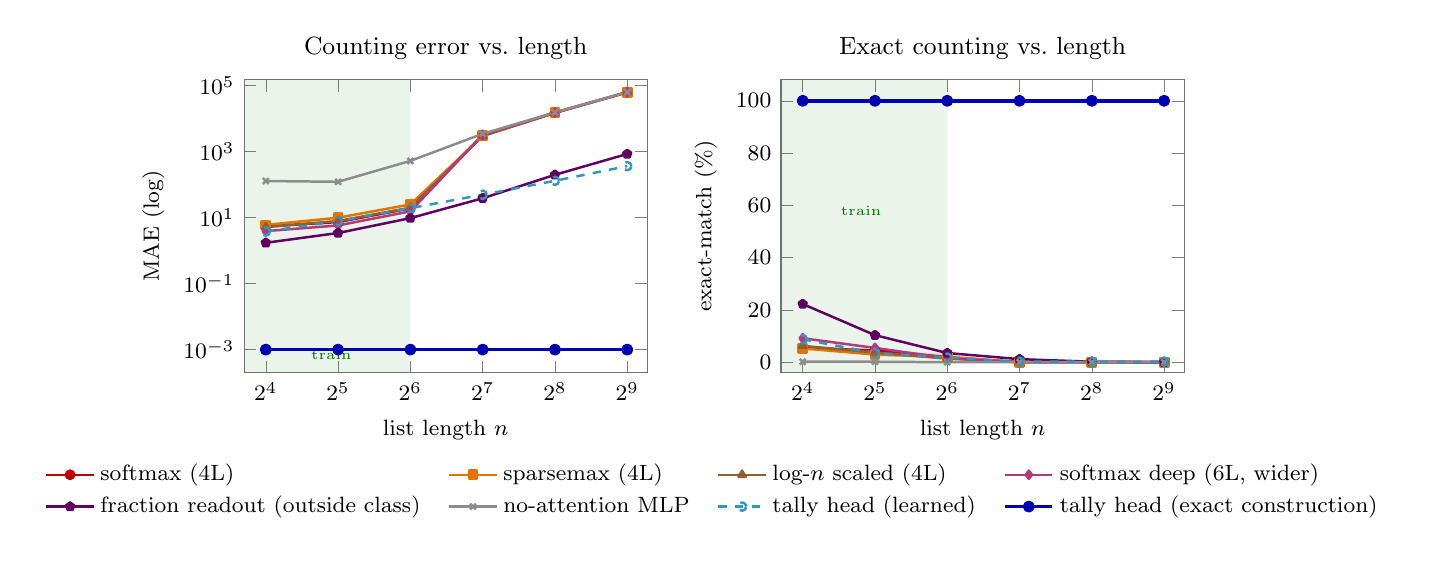
\begin{tikzpicture}
\begin{groupplot}[
  group style={group size=2 by 1, horizontal sep=1.7cm},
  width=6.7cm, height=5.3cm,
  xmode=log, log basis x=2, xmin=13, xmax=620,
  xtick={16,32,64,128,256,512}, xticklabels={$2^4$,$2^5$,$2^6$,$2^7$,$2^8$,$2^9$},
  xlabel={list length $n$},
  tick label style={font=\footnotesize}, label style={font=\footnotesize},
  title style={font=\small,yshift=-2pt}, axis line style={black!55},
  every axis plot/.append style={line join=round},
]
\nextgroupplot[title={Counting error vs.\ length}, ylabel={MAE (log)}, ymin=0.0002, ymax=150000.0, ytick={0.001,0.1,10,1000,100000}, ymode=log, legend cell align=left, legend columns=4, legend to name=toycollapseleg, legend style={font=\footnotesize,draw=none,/tikz/every even column/.append style={column sep=8pt}}]
\addplot[draw=none,fill=green!45!black,opacity=0.08,forget plot] coordinates {(8,0.0002) (64,0.0002) (64,150000.0) (8,150000.0)} \closedcycle;
\addplot[name path=vanillamaehi,draw=none,forget plot] coordinates {(16,5.7024) (32,8.0285) (64,21.8474) (128,3171.2666) (256,15356.4492) (512,63638.4922)};
\addplot[name path=vanillamaelo,draw=none,forget plot] coordinates {(16,5.1728) (32,7.3253) (64,17.6034) (128,3143.4722) (256,15236.0254) (512,63401.625)};
\addplot[red!75!black,opacity=0.13,forget plot] fill between[of=vanillamaehi and vanillamaelo];
\addplot[red!75!black,mark=*,mark size=1.5pt,line width=0.9pt,forget plot] coordinates {(16,5.4017) (32,7.3612) (64,19.2073) (128,3147.0601) (256,15272.4199) (512,63570.8984)};
\addplot[orange!90!black,mark=square*,mark size=1.5pt,line width=0.9pt,forget plot] coordinates {(16,6.0229) (32,9.9738) (64,25.0988) (128,3015.23) (256,15042.8545) (512,63185.1602)};
\addplot[brown!75!black,mark=triangle*,mark size=1.5pt,line width=0.9pt,forget plot] coordinates {(16,5.1552) (32,7.9198) (64,20.0719) (128,2979.6401) (256,15014.3955) (512,63189.9961)};
\addplot[magenta!70!black,mark=diamond*,mark size=1.5pt,line width=0.9pt,forget plot] coordinates {(16,3.9079) (32,5.8023) (64,15.5557) (128,3212.5913) (256,15259.4746) (512,63653.6562)};
\addplot[violet!75!black,mark=pentagon*,mark size=1.5pt,line width=0.9pt,forget plot] coordinates {(16,1.731) (32,3.4243) (64,9.6761) (128,38.7026) (256,198.9484) (512,851.9933)};
\addplot[black!45,mark=x,mark size=1.5pt,line width=0.9pt,forget plot] coordinates {(16,128.8506) (32,122.1136) (64,525.4124) (128,3484.916) (256,15486.6973) (512,63856.4727)};
\addplot[cyan!75!black,dashed,mark=o,mark size=1.5pt,line width=0.9pt,forget plot] coordinates {(16,3.8015) (32,7.8606) (64,19.4043) (128,49.4867) (256,130.9548) (512,364.3456)};
\addplot[blue!70!black,mark=*,mark size=1.5pt,line width=1.3pt,forget plot] coordinates {(16,0.001) (32,0.001) (64,0.001) (128,0.001) (256,0.001) (512,0.001)};
\addlegendimage{red!75!black,mark=*,mark size=1.5pt,line width=0.9pt}\addlegendentry{softmax (4L)}
\addlegendimage{orange!90!black,mark=square*,mark size=1.5pt,line width=0.9pt}\addlegendentry{sparsemax (4L)}
\addlegendimage{brown!75!black,mark=triangle*,mark size=1.5pt,line width=0.9pt}\addlegendentry{log-$n$ scaled (4L)}
\addlegendimage{magenta!70!black,mark=diamond*,mark size=1.5pt,line width=0.9pt}\addlegendentry{softmax deep (6L, wider)}
\addlegendimage{violet!75!black,mark=pentagon*,mark size=1.5pt,line width=0.9pt}\addlegendentry{fraction readout (outside class)}
\addlegendimage{black!45,mark=x,mark size=1.5pt,line width=0.9pt}\addlegendentry{no-attention MLP}
\addlegendimage{cyan!75!black,dashed,mark=o,mark size=1.5pt,line width=0.9pt}\addlegendentry{tally head (learned)}
\addlegendimage{blue!70!black,mark=*,mark size=1.5pt,line width=1.3pt}\addlegendentry{tally head (exact construction)}
\node[font=\tiny,green!45!black] at (axis cs:30,7e-4) {train};
\nextgroupplot[title={Exact counting vs.\ length}, ylabel={exact-match (\%)}, ymin=-4, ymax=108, ytick={0,20,40,60,80,100}]
\addplot[draw=none,fill=green!45!black,opacity=0.08,forget plot] coordinates {(8,-4) (64,-4) (64,108) (8,108)} \closedcycle;
\addplot[name path=vanillaexacthi,draw=none,forget plot] coordinates {(16,6.25) (32,4.8828) (64,3.125) (128,0.0) (256,0.0) (512,0.0)};
\addplot[name path=vanillaexactlo,draw=none,forget plot] coordinates {(16,4.6875) (32,3.125) (64,1.3672) (128,0.0) (256,0.0) (512,0.0)};
\addplot[red!75!black,opacity=0.13,forget plot] fill between[of=vanillaexacthi and vanillaexactlo];
\addplot[red!75!black,mark=*,mark size=1.5pt,line width=0.9pt,forget plot] coordinates {(16,5.4688) (32,4.4922) (64,1.9531) (128,0.0) (256,0.0) (512,0.0)};
\addplot[orange!90!black,mark=square*,mark size=1.5pt,line width=0.9pt,forget plot] coordinates {(16,5.2734) (32,2.9297) (64,1.9531) (128,0.0) (256,0.0) (512,0.0)};
\addplot[brown!75!black,mark=triangle*,mark size=1.5pt,line width=0.9pt,forget plot] coordinates {(16,6.25) (32,3.7109) (64,1.3672) (128,0.0) (256,0.0) (512,0.0)};
\addplot[magenta!70!black,mark=diamond*,mark size=1.5pt,line width=0.9pt,forget plot] coordinates {(16,9.1797) (32,5.4688) (64,1.5625) (128,0.0) (256,0.0) (512,0.0)};
\addplot[violet!75!black,mark=pentagon*,mark size=1.5pt,line width=0.9pt,forget plot] coordinates {(16,22.2656) (32,10.3516) (64,3.5156) (128,1.1719) (256,0.1953) (512,0.0)};
\addplot[black!45,mark=x,mark size=1.5pt,line width=0.9pt,forget plot] coordinates {(16,0.1953) (32,0.1953) (64,0.0) (128,0.0) (256,0.0) (512,0.0)};
\addplot[cyan!75!black,dashed,mark=o,mark size=1.5pt,line width=0.9pt,forget plot] coordinates {(16,8.7891) (32,3.5156) (64,1.7578) (128,0.1953) (256,0.1953) (512,0.1953)};
\addplot[blue!70!black,mark=*,mark size=1.5pt,line width=1.3pt,forget plot] coordinates {(16,100.0) (32,100.0) (64,100.0) (128,100.0) (256,100.0) (512,100.0)};
\node[font=\tiny,green!45!black] at (axis cs:28,58) {train};
\end{groupplot}
\coordinate (leg) at ($(group c1r1.south)!0.5!(group c2r1.south)$);
\node[anchor=north] at ([yshift=-0.9cm]leg) {\pgfplotslegendfromname{toycollapseleg}};
\end{tikzpicture}

\caption{The ablation ladder of Table~\ref{tab:ablations}, run out to
$n=512$. Shaded region is the training range. Left: mean absolute error.
Right: exact match. Every normalized variant tracks the truth inside the
training range and then leaves it. Sharper attention (sparsemax), sharper
with length ($\log n$-scaled), more depth and width, and rescaling the
output after the fact (fraction readout) all fail in the same way, which
is what Theorem~\ref{thm:barrier} predicts, since none of them enlarges an
average. The no-attention MLP fails everywhere, which confirms the task
genuinely needs pairwise comparison. The hand-built tally head is flat at
the bottom left and at $100\%$ on the right, at every length, with no
training.}
\label{fig:collapse}
\end{figure}

Figure~\ref{fig:collapse} is the first three steps of the experimental
logic in Section~\ref{sec:ablation}: a normal Transformer out of range,
then sharper attention, then a bigger model, all three failing. Each one
fits comfortably inside the training range first, which is the control that
rules out under-training.

\subsection{The denominator control}
\label{sec:denom}

The fourth step needs its own figure, because it identifies the cause.

\begin{figure}[htbp]
\centering
% Auto-generated by experiments/make_denominator_pgf.py -- PGFPlots denominator control.
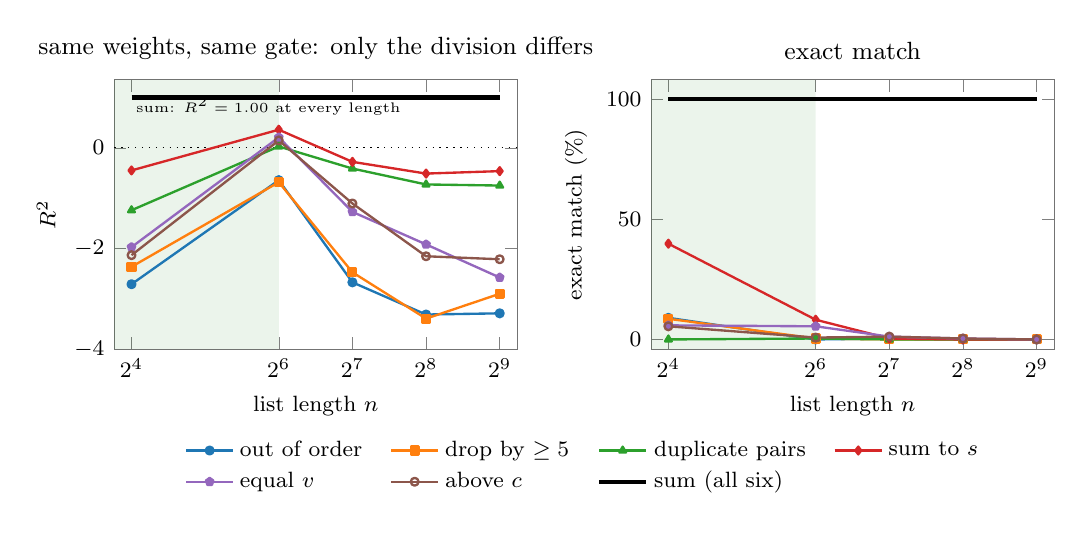
\begin{tikzpicture}
\definecolor{den0}{RGB}{31,119,180}
\definecolor{den1}{RGB}{255,127,14}
\definecolor{den2}{RGB}{44,160,44}
\definecolor{den3}{RGB}{214,39,40}
\definecolor{den4}{RGB}{148,103,189}
\definecolor{den5}{RGB}{140,86,75}
\begin{groupplot}[
  group style={group size=2 by 1, horizontal sep=1.7cm},
  width=6.7cm, height=5.0cm,
  xmode=log, log basis x=2, xmin=13.6, xmax=604.16,
  xtick={16,64,128,256,512}, xticklabels={$2^{4}$,$2^{6}$,$2^{7}$,$2^{8}$,$2^{9}$},
  xlabel={list length $n$},
  tick label style={font=\footnotesize}, label style={font=\footnotesize},
  title style={font=\small,yshift=-2pt}, axis line style={black!55},
  every axis plot/.append style={line join=round},
]
\nextgroupplot[title={same weights, same gate: only the division differs}, ylabel={$R^2$}, ymin=-4, ymax=1.35, legend cell align=left, legend columns=4, legend to name=denleg, legend style={font=\footnotesize,draw=none,/tikz/every even column/.append style={column sep=8pt}}]
\addplot[draw=none,fill=green!45!black,opacity=0.08,forget plot] coordinates {(8,-4) (64,-4) (64,1.35) (8,1.35)} \closedcycle;
\addplot[black,dotted,line width=0.5pt,forget plot] coordinates {(13.6,0) (604.16,0)};
\addplot[den0,mark=*,mark size=1.4pt,line width=0.85pt,forget plot] coordinates {(16,-2.71129) (64,-0.643947) (128,-2.67342) (256,-3.31379) (512,-3.28997)};
\addplot[den1,mark=square*,mark size=1.4pt,line width=0.85pt,forget plot] coordinates {(16,-2.36533) (64,-0.684384) (128,-2.47404) (256,-3.39494) (512,-2.9011)};
\addplot[den2,mark=triangle*,mark size=1.4pt,line width=0.85pt,forget plot] coordinates {(16,-1.24107) (64,0.0266132) (128,-0.412743) (256,-0.728629) (512,-0.749976)};
\addplot[den3,mark=diamond*,mark size=1.4pt,line width=0.85pt,forget plot] coordinates {(16,-0.449927) (64,0.359717) (128,-0.279448) (256,-0.51228) (512,-0.463423)};
\addplot[den4,mark=pentagon*,mark size=1.4pt,line width=0.85pt,forget plot] coordinates {(16,-1.97419) (64,0.207317) (128,-1.27338) (256,-1.91997) (512,-2.57791)};
\addplot[den5,mark=o,mark size=1.4pt,line width=0.85pt,forget plot] coordinates {(16,-2.13416) (64,0.146103) (128,-1.10668) (256,-2.15566) (512,-2.2152)};
\addplot[black,line width=1.6pt,forget plot] coordinates {(16,1) (64,1) (128,1) (256,1) (512,1)};
\node[anchor=north west,font=\tiny] at (rel axis cs:0.03,0.97) {sum: $R^2=1.00$ at every length};
\addlegendimage{den0,mark=*,mark size=1.4pt,line width=0.85pt}\addlegendentry{out of order}
\addlegendimage{den1,mark=square*,mark size=1.4pt,line width=0.85pt}\addlegendentry{drop by $\geq5$}
\addlegendimage{den2,mark=triangle*,mark size=1.4pt,line width=0.85pt}\addlegendentry{duplicate pairs}
\addlegendimage{den3,mark=diamond*,mark size=1.4pt,line width=0.85pt}\addlegendentry{sum to $s$}
\addlegendimage{den4,mark=pentagon*,mark size=1.4pt,line width=0.85pt}\addlegendentry{equal $v$}
\addlegendimage{den5,mark=o,mark size=1.4pt,line width=0.85pt}\addlegendentry{above $c$}
\addlegendimage{black,line width=1.6pt}\addlegendentry{sum (all six)}
\nextgroupplot[title={exact match}, ylabel={exact match (\%)}, ymin=-4, ymax=108]
\addplot[draw=none,fill=green!45!black,opacity=0.08,forget plot] coordinates {(8,-4) (64,-4) (64,108) (8,108)} \closedcycle;
\addplot[den0,mark=*,mark size=1.4pt,line width=0.85pt,forget plot] coordinates {(16,8.98438) (64,0) (128,0.390625) (256,0) (512,0)};
\addplot[den1,mark=square*,mark size=1.4pt,line width=0.85pt,forget plot] coordinates {(16,8.59375) (64,0.390625) (128,0) (256,0) (512,0)};
\addplot[den2,mark=triangle*,mark size=1.4pt,line width=0.85pt,forget plot] coordinates {(16,0) (64,0.390625) (128,0) (256,0) (512,0)};
\addplot[den3,mark=diamond*,mark size=1.4pt,line width=0.85pt,forget plot] coordinates {(16,39.8438) (64,8.20312) (128,0.390625) (256,0) (512,0)};
\addplot[den4,mark=pentagon*,mark size=1.4pt,line width=0.85pt,forget plot] coordinates {(16,5.85938) (64,5.46875) (128,1.17188) (256,0.390625) (512,0)};
\addplot[den5,mark=o,mark size=1.4pt,line width=0.85pt,forget plot] coordinates {(16,5.46875) (64,0.78125) (128,1.17188) (256,0.390625) (512,0)};
\addplot[black,line width=1.6pt,forget plot] coordinates {(16,100) (64,100) (128,100) (256,100) (512,100)};
\end{groupplot}
\coordinate (leg) at ($(group c1r1.south)!0.5!(group c2r1.south)$);
\node[anchor=north] at ([yshift=-0.9cm]leg) {\pgfplotslegendfromname{denleg}};
\end{tikzpicture}

\caption{The single decisive control. Same weights, same clamp gate, same
votes. The only difference is whether the votes are summed or divided by
the number of pairs. Summing gives $R^2 = 1.00$ at every length, the flat
line at the top of both panels. Dividing collapses all six questions. If
the barrier were about attention, or depth, or the task being hard, this
figure would not look like this.}
\label{fig:denominator}
\end{figure}

Figure~\ref{fig:denominator} is the experiment we would keep if we could
only keep one. Everything is held fixed except the denominator. Normalized
collapses, un-normalized does not, and there is nothing else left to
attribute the difference to.

\subsection{Frozen Qwen: three heads on the same features}
\label{sec:qwen-setup}

Having established that the tally head is essential for a vanilla
Transformer, we now test on a real base Transformer released by a major
laboratory: Qwen3-0.6B, a $28$-layer pretrained language model from the
Alibaba Qwen team \citep{qwen3}. The key point is that we freeze all Qwen weights, read
the same internal features, and change only the small output/aggregation
head, so that we can isolate the one difference that matters: average
versus sum.

The tally head is intended as an extra architectural component alongside
the normal Transformer. We do not rewrite Qwen internally; we attach the
tally head to Qwen's layer-$14$ hidden states. We choose layer $14$ not
because it is the optimal layer for this particular model, but because it
gives Qwen fourteen layers in which to process the English question and
the list. The whole thing is a single forward pass. A representative
prompt is:

\begin{quote}
\ttfamily
Question: How many pairs are out of order?\\
List: 5 2 9 7 3\\
Answer:
\end{quote}

We choose three experiments:
\begin{itemize}
\item \textbf{Experiment A:} frozen Qwen $+$ value head.
\item \textbf{Experiment B:} frozen Qwen $+$ mean-pool head.
\item \textbf{Experiment C:} frozen Qwen $+$ tally head.
\end{itemize}
We do not put all three inside the same Qwen at once. We run them one by
one and compare:

\begin{quote}
Prompt and list $\rightarrow$ frozen Qwen, up to layer $14$ $\rightarrow$
list-token hidden vectors $h_1, h_2, \dots, h_n$ $\rightarrow$ choose
\emph{one} add-on head $\rightarrow$ predicted count.
\end{quote}

\subsubsection*{The three heads}

For a prompt containing a list, frozen Qwen produces hidden vectors for
the list tokens, $h_1, h_2, \dots, h_{\text{last}}$. Qwen is frozen; we
train only the small added head.

\paragraph{A. Value head.}
\begin{equation}
\hat{y} \;=\; w^{\top} h_{\text{last}} + b .
\label{eq:valuehead}
\end{equation}
It takes \emph{one} hidden vector, the final answer-position vector, and
uses a linear layer to predict a count. It asks one vector to somehow
hold the whole answer. We include it because it represents the normal
Transformer strategy: put the answer into one final hidden state, then
read it out. The normal architecture's output layer produces vocabulary
logits and a next token; here it produces a predicted count instead.

\paragraph{B. Mean-pool head.}
First average all list-token vectors, then read out a number:
\begin{equation}
\bar{h} = \frac{1}{n}\sum_{i=1}^{n} h_i,
\qquad
\hat{y} = w^{\top}\bar{h} + b .
\label{eq:meanpool}
\end{equation}
We include it because it is the clean average-versus-sum control. It uses
every list token, but averages their evidence instead of adding it.

\paragraph{C. Tally head.}
For inversion-like pair counting,
\begin{equation}
q_i = W_Q h_i, \quad k_j = W_K h_j, \quad
\text{vote}_{ij} = \clampf(q_i \cdot k_j, 0, 1), \quad
\hat{y} = \sum_{j<i} \text{vote}_{ij}.
\label{eq:qwen-tally}
\end{equation}
We include it because it is the proposed additive alternative. Unlike
mean-pool, it does not divide the total by $n$ or by the number of pairs.



\subsubsection*{What is frozen and what is learned}

Frozen: all Qwen parameters. Learned: only the small attached head, meaning
$w, b$ for the value head; $w, b$ for the mean head; and $W_Q$, $W_K$ plus
small output parameters for the tally head. Therefore, if the tally head
performs better, it is \emph{not} because it had a better language model.
All three use exactly the same Qwen representations. Its key difference is
only this: local comparisons $\rightarrow$ votes $\rightarrow$ sum.

For each list: Qwen processes the prompt once; we extract the chosen
hidden states, mainly from layer $14$; and the attached head outputs one
numerical count. There is no chain of thought, no repeated prompting, and
no external counting program.

\begin{remark}[Why layer 14, and not layer 1]
\label{rem:layer14}
The reason we attach at layer $14$ and immediately count there is not that
layers $1$ to $14$ keep one kind of information and layers $15$ to $28$ keep
another. We could attach the tally head to the first layer and that would
be perfectly fine, but in that case the rule is already known, the head
can compare raw digit features immediately, and it does not need Qwen at
all. That is our hand-built construction. When the Qwen experiment asks a
question in English, the model needs some layers to actually process and
understand it before the gate layer. One of our conjectures is that every
different model has a different optimal layer at which to add the tally
head. Layer $14$ is the chosen mid-stack tap for the main control
experiment; it is not a universal best placement.
\end{remark}

\label{sec:extrap}

We want the model not only to learn how to count but also to generalize.
The head is trained on $n \in \{4, 5, \dots, 16\}$, where $n$ is the list
length, so a list can hold four numbers, five numbers, and so on. Then,
without changing any weights, we test it on lists up to $n = 96$. The
central question is therefore: if the model learns on lists of at most
$16$ items, can it still count correctly on a list of $96$ items? This is
length extrapolation, or out-of-distribution (OOD) generalization.

For example, at the largest training length there are
\[
\binom{16}{2} = 120
\]
possible pairs with $j < i$, but at test length there are
\[
\binom{96}{2} = 4560 .
\]
So a model tested at $n = 96$ must handle about $38$ times more possible
pairs than at $n = 16$.

\begin{remark}[Pairwise versus item-wise, restated]
\label{rem:pair-vs-item}
The reason we want $\binom{n}{2}$ is that inversion counting is a
\emph{pairwise} task. For a list of length $4$ the pairs to check are
$(1,2), (1,3), (1,4), (2,3), (2,4), (3,4)$, so $\binom{4}{2} = 6$. For
each pair we ask whether the earlier value is bigger than the later value,
then add the yes-votes. For length $16$ there are up to $\binom{16}{2} =
120$ possible pairs to check, which does \emph{not} mean every list has
$120$ inversions. A sorted list has $0$; a reverse-sorted list with all
distinct values has $120$; most lists are somewhere in between. An
\emph{item-wise} task, such as counting how many $7$s are in a list of
length $16$, requires going through only $16$ items, so the count length
is just $n$. For $n = 16$: item-wise maximum count is $16$; pairwise
maximum possible pair count is $120$.
\end{remark}

\label{sec:controls}

\paragraph{Control 1: preventing ``guess the typical count for this
length''.}
A model could fake success by learning the typical answer for a given list
length instead of reading the list. To prevent this, the dataset includes a
wide range of true counts at every fixed length. For example, two lists can
both have length $96$ but very different answers, one with a true answer
of $10$ and another with a true answer of $300$. A length-only prediction
cannot solve both.

\paragraph{Control 2: the null baseline.}
We compare the model against a content-blind baseline that ignores the list
and always predicts the typical count:
\[
\hat{y}_{\text{null}} = \text{average true count at that test length},
\qquad\text{which is where } R^2 = 0 .
\]
If $R^2 \leq 0$, the model performs no better than this baseline, or it
performs worse. This is what makes the negative $R^2$ values of the value and
mean heads meaningful: at long lengths they perform worse than simply
predicting the average count for a length-$96$ list.

\paragraph{Control 3: fixed-length correlation between prediction and truth.}
Keep the list length fixed at $n = 96$, then test the model on many
different length-$96$ lists whose true counts differ because their
contents differ. For each list, record (prediction, true count), then
compute the Pearson correlation $\corr(\hat{y}, y)$ over that set. This asks:
\emph{among lists of exactly the same length, does the model predict a
larger answer when the true answer is larger?} A high correlation
therefore shows that the model is responding to the \emph{contents} of the
list, not just its length.

\paragraph{Reading the tables.} In the theorems \emph{exact} means the
head's real-valued output equals the count. In the tables \emph{exact
match} means it does so after rounding to the nearest integer. The two come
apart more often than you would expect: a high $R^2$ with no exact matches
at all is possible, and does happen, when the prediction tracks which lists
have larger counts while never landing on an integer. That is a resolution
failure, and it is not counting.

%=======================================================================
\subsection{One tally head per task}
\label{sec:per-task}

This is our first Qwen experiment, and it is not yet the single universal
English-question head. It asks a simpler question first: can the frozen
Qwen features support a learned additive head for each individual counting
rule?

\begin{table}[htbp]
\centering
\caption{Per-task heads on frozen Qwen3-0.6B. Trained on $n \leq 16$,
tested at $n = 96$. ``Corr'' is the fixed-length control from Control 3,
measured across many different lists that all have length $96$. Value and
mean heads are negative everywhere at $n = 96$, meaning they do worse than
predicting the average count.}
\label{tab:pertask}
\small
\begin{tabular}{@{}llrrrrrr@{}}
\toprule
\textbf{Question} & \textbf{What it counts} &
\textbf{Tally $R^2$} & \textbf{Tally $R^2$} & \textbf{Tally} & \textbf{Tally} &
\textbf{Value} & \textbf{Mean} \\
 & & \textbf{$n=16$} & \textbf{$n=96$} & \textbf{corr} & \textbf{exact} &
\textbf{$R^2$} & \textbf{$R^2$} \\
\midrule
Inversions      & earlier number $>$ later number      & 1.00 & 0.96  & 0.99 & 3\%  & $-3.2$ & $-3.2$ \\
Drops $\geq 5$  & earlier number at least 5 bigger     & 0.85 & 0.79  & 0.96 & 1\%  & $-2.4$ & $-2.3$ \\
Duplicate pairs & earlier number $=$ later number      & 0.98 & 0.95  & 0.98 & 0\%  & $-1.7$ & $-1.7$ \\
Pairs sum to $s$& two numbers add to target $s$        & 0.09 & $-1.93$ & 0.45 & 0\% & $-0.9$ & $-0.9$ \\
Equal to $v$    & individual items equal target digit $v$ & 1.00 & 1.00 & 1.00 & 98\% & $-1.8$ & $-1.7$ \\
Above $c$       & individual items greater than threshold $c$ & 1.00 & 1.00 & 1.00 & 79\% & $-2.2$ & $-1.8$ \\
\bottomrule
\end{tabular}
\end{table}

The tally head tracks long inversion counts very well, but it usually does
not land on the exact integer. It learned an approximate, length-stable counting rule of its own, not the exact one we wrote by hand. The headline
finding is this: the same frozen Qwen representations can support
extrapolating inversion counts when we \emph{add} votes, but not when we
read out through one vector or through an average.

The key thing to identify for ``pairs sum to $s$'' is that the $R^2$ was
already very poor at the training length of $16$. The small learned tally
head never successfully learned a pair-sum predicate from frozen Qwen
layer-$14$ vectors in the first place. That is an optimization and
representation limitation, not a limitation of the tally architecture or
of Theorem~\ref{thm:universal}, and the distinction matters.



\subsection{One shared head that reads the question}
\label{sec:shared}

We can now say that the tally head architecture is fundamentally correct,
with empirical results backing it up. Up to this point we used one
separate tally head per task: one head trained for ``how many $3$s'', a
different head trained for ``how many numbers above $2$''. Each head
already knows its rule through its learned weights.

Now we test a harder question. Can \emph{one shared} tally head read the
question in the prompt and count the requested thing? That is, one set of
tally head weights, reused across many differently worded questions.

It was trained on only two question forms: ``how many $3$s?'' and ``how
many numbers are above $2$?''. It was never trained on ``how many $7$s?'',
``how many $8$s?'', ``how many $9$s?'', or ``how many numbers are above
$4$?''. It still tests at $n = 96$ after training only up to $n = 16$.

Before the numbers, We should be careful about what ``one shared head''
means here, because the phrase can be read as claiming more than we can show. The head does carry one shared bilinear gate and one shared item
gate, and those are what read the ``$7$'' or the ``above $4$'' out of the
question text and point the counting at the right items. Alongside them it
also carries a small set of parameters attached to each grammatical type,
a gate block, two biases and an output affine, and the type index saying
whether this is an item question or a pair question is something we hand the model. It does not work that out from the words. So what is
actually being shown is generalization to new target values inside a
grammatical type. New digits, a new threshold, at six times the training
length. It is not a head that reads an unfamiliar English sentence and
figures out its grammatical form. Taking the type index away and making the
head route itself from the text alone is the obvious next thing to try and we have not tried it.

\begin{table}[htbp]
\centering
\caption{One shared tally head, taking the question in plain English.
``Within 10\%'' is the fraction of test lists whose prediction lands
within ten percent of the true count. ``Successful seeds'' counts how many
of five random seeds trained successfully.}
\label{tab:shared}
\small
\begin{tabular}{@{}lcrrcr@{}}
\toprule
\textbf{Question} & \textbf{Seen in training?} & \textbf{Tally $R^2$} &
\textbf{Within 10\%} & \textbf{Successful seeds} & \textbf{Value-head $R^2$} \\
\midrule
how many 3s?                  & yes & 0.94 & 53\% & 5/5 & $-1.8$ \\
how many numbers above 2?     & yes & 0.90 & 55\% & 5/5 & $-2.2$ \\
how many 7s?                  & no  & 0.92 & 50\% & 4/5 & \\
how many 8s?                  & no  & 0.89 & 42\% & 4/5 & \\
how many 9s?                  & no  & 0.84 & 34\% & 5/5 & \\
how many numbers above 4?     & no  & 0.89 & 36\% & 5/5 & \\
\bottomrule
\end{tabular}
\end{table}


\begin{figure}[htbp]
\centering
% Auto-generated by experiments/make_sixquestions_pgf.py -- PGFPlots summary bars.
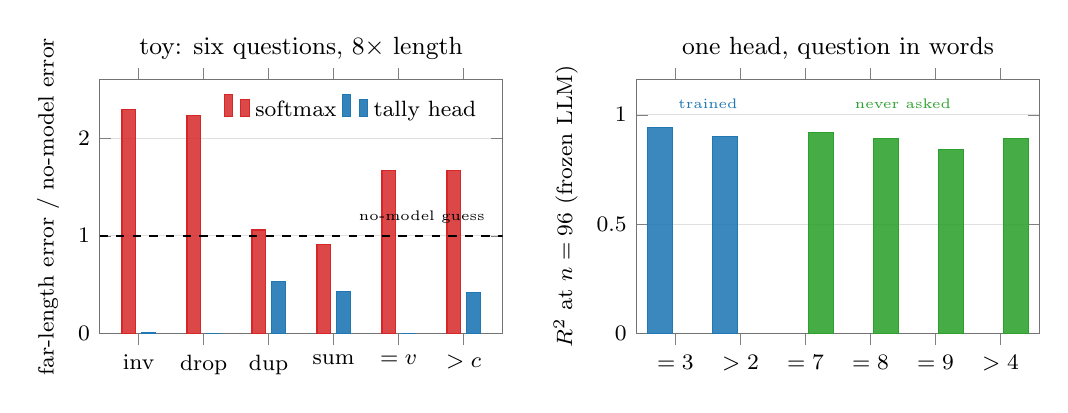
\begin{tikzpicture}
\definecolor{sqred}{RGB}{214,39,40}
\definecolor{sqblue}{RGB}{31,119,180}
\definecolor{sqgreen}{RGB}{44,160,44}
\begin{groupplot}[
  group style={group size=2 by 1, horizontal sep=1.7cm},
  width=6.7cm, height=4.8cm,
  ybar, /pgf/bar width=5pt, enlarge x limits=0.12,
  tick label style={font=\footnotesize}, label style={font=\footnotesize},
  title style={font=\small,yshift=-2pt}, axis line style={black!55},
  ymajorgrids, grid style={black!12},
]
\nextgroupplot[title={toy: six questions, $8\times$ length},
  ylabel={far-length error / no-model error}, ymin=0, ymax=2.6,
  xtick={0,1,2,3,4,5}, xticklabels={inv,drop,dup,sum,$=v$,$>c$},
  legend cell align=left, legend columns=2,
  legend style={font=\footnotesize,draw=none,at={(0.97,0.97)},anchor=north east}]
\addplot[draw=sqred,fill=sqred,fill opacity=0.85] coordinates {(0,2.3) (1,2.23) (2,1.06) (3,0.91) (4,1.67) (5,1.67)};
\addlegendentry{softmax}
\addplot[draw=sqblue,fill=sqblue,fill opacity=0.9] coordinates {(0,0.01) (1,0.001) (2,0.53) (3,0.43) (4,0) (5,0.42)};
\addlegendentry{tally head}
\draw[dashed,black,line width=0.7pt] (rel axis cs:0,0.3846) -- (rel axis cs:1,0.3846);
\node[anchor=south east,font=\tiny] at (rel axis cs:0.98,0.395) {no-model guess};
\nextgroupplot[title={one head, question in words},
  ylabel={$R^2$ at $n=96$ (frozen LLM)}, ymin=0, ymax=1.16,
  xtick={0,1,2,3,4,5}, xticklabels={$=3$,$>2$,$=7$,$=8$,$=9$,$>4$}, /pgf/bar width=9pt]
\addplot[draw=sqblue,fill=sqblue,fill opacity=0.88] coordinates {(0,0.94) (1,0.9)};
\addplot[draw=sqgreen,fill=sqgreen,fill opacity=0.88] coordinates {(2,0.92) (3,0.89) (4,0.84) (5,0.89)};
\node[font=\tiny,sqblue] at (axis cs:0.5,1.05) {trained};
\node[font=\tiny,sqgreen] at (axis cs:3.5,1.05) {never asked};
\end{groupplot}
\end{tikzpicture}

\caption{Left: the toy, six questions, error relative to the no-model
baseline (the dashed line at $1.0$ is what you get by ignoring the list).
Softmax is at or above that line on four of the six. Right: the shared
head on frozen Qwen, $R^2$ at $n=96$. The two blue bars are the question
forms it was trained on. The four green bars are questions it was never
asked during training. Getting ``how many sevens'' right after only ever
being trained on ``how many threes'' is the part that is hard to explain
as memorization.}
\label{fig:sixquestions}
\end{figure}

This table is our strongest finding. It is not merely that the head counts
$3$s. It also answers questions about $7$, $8$, and $9$, none of which were
included in training, and it generalizes to them. That is exactly the
evidence that the shared head did not memorize a small lookup table of the
form ``question A, use rule A; question B, use rule B''. It learned a more
general pattern: read which condition the English question specifies,
identify the list items satisfying it, and add their votes.

\subsubsection*{Scope of this result}

There are three things this supports. The head is not memorizing one digit, since it
learned from $3$ and still handles $7$, $8$ and $9$. Frozen Qwen carries the
question into the list-item representations, since the same shared head
behaves differently when the prompt names a different target. And
unnormalized addition still works at $n = 96$, six times the longest
training list.

And three things it does not. It is not exact counting at every length; $R^2$ is
high, and that is not the same as claiming the learned head counts
perfectly forever. It does not show that every pairwise question can be
learned jointly, because pair-sum failed and shared multi-rule pairwise
training was not reliable, though neither contradicts
Theorem~\ref{thm:universal}, which says suitable weights exist and promises
nothing about SGD finding one shared set of them from frozen features. And
it says nothing about whether ordinary language models can count with chain
of thought or with a calculator attached, since the claim is about a
single-pass fixed readout and only that.

So the claim we will defend is this. A small additive head on frozen Qwen
features substantially improves length extrapolation and generalizes to
item-count questions nobody trained it on, and optimization and
representation limits remain on the harder pairwise ones.

\subsection{Probing layer 14}
\label{sec:probe}

\subsubsection*{Probe 1: is the local evidence there at all?}

From the Qwen technical report \citep{qwen3} we know that the model has $28$ layers, but
we do not automatically know which layer contains the most useful
representation for the small tally head, or which part handles arithmetic.
So we built a feature probe. Its role is to ask: from the hidden vectors
at this layer, can a simple classifier recognize the local rule we need?

The probe is not part of Qwen and not part of the final tally head. It is a
tiny logistic classifier,
\begin{equation}
p_i \;=\; \sigma\!\left(w^{\top}\LN(h_i) + b\right),
\label{eq:probe}
\end{equation}
where $h_i$ is Qwen's frozen hidden vector for item $i$, $w$ and $b$ are the
only new parameters, and $p_i$ is its estimated probability that item $i$
has the property we are asking about. If it succeeds we say the information
is \emph{linearly accessible} at that layer, and that matters because a
tally-head failure has two possible causes: Qwen did not keep the
information, which is an architecture problem, or Qwen kept it and the head
failed to use it, which is an aggregation or optimization problem. The probe
is what tells those two apart.

We ran the probe against three representative layers, $7$, $14$, and $21$.
Most rules were easily readable at all three sampled layers; pair-sum was
consistently weaker; and layer $14$ is a reasonable middle choice, not a tuned one.

For pairwise tasks, the probe does not try to count all the pairs. For
each position $i$ it only asks: does this item close at least one valid
pair with something earlier?

\begin{example}[Probe labels for the list $5, 2, 9, 3$]
\label{ex:probe}
\begin{center}
\begin{tabular}{@{}rll@{}}
\toprule
\textbf{Later item} & \textbf{Is there an earlier bigger number?} & \textbf{Probe label} \\
\midrule
5 & no earlier item                     & 0 \\
2 & yes: $5 > 2$                        & 1 \\
9 & no earlier number bigger than 9     & 0 \\
3 & yes: $5 > 3$, and also $9 > 3$      & 1 \\
\bottomrule
\end{tabular}
\end{center}
\noindent The probe labels are $[0, 1, 0, 1]$. Note that the true inversion
count is $3$, but the probe labels sum to only $2$. That is fine: the probe
is \emph{not} counting inversions. It only checks whether Qwen's hidden
vector at each position contains evidence that the item participates in at
least one valid pair with $j < i$.
\end{example}

\begin{table}[htbp]
\centering
\caption{Probe ROC AUC by layer. Pair-sum is the weakest row at every
layer.}
\label{tab:auc}
\begin{tabular}{@{}lrrr@{}}
\toprule
\textbf{Question} & \textbf{Layer 7} & \textbf{Layer 14} & \textbf{Layer 21} \\
\midrule
Inversions       & 0.991 & 0.980 & 0.997 \\
Drops $\geq 5$   & 0.994 & 0.995 & 0.997 \\
Duplicate pairs  & 1.000 & 1.000 & 1.000 \\
Pairs sum to $s$ & 0.916 & 0.899 & 0.904 \\
Equal to $v$     & 1.000 & 1.000 & 1.000 \\
Above $c$        & 1.000 & 1.000 & 1.000 \\
\bottomrule
\end{tabular}
\end{table}

Qwen's frozen representations therefore contain highly readable local
evidence for most counting predicates. Pair-sum is the weakest, and none of
these AUC scores alone prove that Qwen can aggregate that evidence into an
unbounded count. Recall that $\mathrm{AUC} = 0.98$ means that if we choose
one item with label $1$ and one item with label $0$, the probe gives the
positive item a higher score about $98\%$ of the time.

\subsubsection*{Probe 2: can one final-token vector carry the total count?}

For the second probe we ask a different question: can we read the whole
numerical count out of one final-token vector? It uses the standard simple
readout
\begin{equation}
\hat{y} \;=\; w^{\top} h_{\text{last}},
\label{eq:probe2}
\end{equation}
where $h_{\text{last}}$ is Qwen's final-token hidden vector, $w$ is a
small learned vector, and $\hat{y}$ is the predicted total count. This is
essentially a very simple value-head probe. We train $w$ on short lists,
$n = 4$ to $16$, then evaluate at $n = 16$, $48$, and $96$. Because this
probe predicts a numerical value such as $37$, we evaluate it with $R^2$.

\begin{table}[htbp]
\centering
\caption{Final-token probe. Every row is negative by $n = 48$.}
\label{tab:probe2}
\begin{tabular}{@{}lrrr@{}}
\toprule
\textbf{Question} & \textbf{$R^2$, $n=16$} & \textbf{$R^2$, $n=48$} & \textbf{$R^2$, $n=96$} \\
\midrule
Inversions       & 0.623 & $-3.003$ & $-2.969$ \\
Drops $\geq 5$   & 0.597 & $-1.210$ & $-1.916$ \\
Duplicate pairs  & 0.828 & $-1.491$ & $-1.887$ \\
Pairs sum to $s$ & 0.138 & $-0.504$ & $-0.860$ \\
Equal to $v$     & 0.896 & $-1.720$ & $-1.527$ \\
Above $c$        & 0.849 & $-2.097$ & $-2.443$ \\
\bottomrule
\end{tabular}
\end{table}

This table shows that for most tasks the final-token probe can predict
counts at short lengths such as $n = 16$, but by $n = 48$ and $n = 96$
every row has negative $R^2$. Qwen's item vectors can contain highly
readable local evidence, and yet a standard one-vector readout cannot turn
that evidence into a growing total as the list becomes longer. This is
without the tally head. A side note on terminology: \emph{local evidence}
means information about one small part of the list, not the final total.

\subsection{Training robustness and active-region initialization}
\label{sec:robustness}

We now examine a factual point about the tally head: it can still fail to
\emph{train}. Theorem~\ref{thm:universal} says that a suitable set of
weights exists for every fixed counting rule. It does not say that
gradient descent will always find them.

Throughout our examination, the main practical failure came from the
design of the clamp, $v = \clampf(\ell, 0, 1)$. Outside the middle region
$[0,1]$ the clamp is flat, and its gradient is zero. So if the random
initialization makes most scores land outside that region, then either
every vote becomes $0$ (all scores negative) or every vote becomes $1$
(all scores above one), and learning gets stuck because the gate has
little or no gradient to adjust itself.

The clamp itself is a fixed rule and is never trained. Its derivative is
$1$ on $(0,1)$ and $0$ everywhere else, so a score inside that band leaves
the gate able to learn and a score outside it leaves the gate dead. What
training actually learns is the score,
\begin{equation}
\ell_{ij} \;=\; (W_Q h_i)^{\top}(W_K h_j) + \beta,
\label{eq:learned-logit}
\end{equation}
with learned $W_Q$, $W_K$ and $\beta$, after which the pipeline is clamp,
sum, count. The trouble is entirely at the start: random weights have no
reason to place $\ell_{ij}$ inside a band that narrow, so most scores begin
in a flat region, every vote comes out $0$ or every vote comes out $1$, and
nothing can move toward the right decision because there is no gradient to
move along.

\subsubsection*{The fix: active-region initialization}

The fix, which we call \emph{active-region initialization}, happens once,
after random initialization but before SGD training begins. For each
random seed:
\begin{enumerate}
\item Randomly initialize $W_Q$, $W_K$, and $\beta$.
\item Pass a small calibration batch through the frozen Qwen model.
\item Compute the initial raw scores using
  Eq.~\eqref{eq:learned-logit}.
\item Rescale $W_Q$ and $W_K$ so that the scores are not too widely spread
  out.
\item Shift each question type's bias $\beta$ so that the scores are
  centred near $\ell_{ij} \approx 0.5$.
\item Calibrate the final output scale $c$, then begin ordinary SGD
  training.
\end{enumerate}

Steps 4 and 5 are what the result is really about, and they only ever look
at the features. One batch goes through the frozen model, the scores that
come out are moved into the live band using nothing but their mean and
spread, and the labels for that batch are generated and thrown away because
none of the arithmetic needs them. That matters, since the claim is that a
hard clamp can be made trainable without knowing any answers in advance.

Step 6 is different, and we want to be straight about it. Calibrating the
output scale $c$ does use a training label, the average count in the
calibration batch, in the ordinary way people normalize a regression target
before training. It changes how quickly training converges; whether the
gate is alive at all is settled by steps 4 and 5. It would be easy to run
the two together and call the whole thing label-free, and that would not be
true, so we separate them here. The principle is to place enough gates
inside the active region before training. Once training is under way they
are free to saturate to $0$ or $1$.

\begin{table}[htbp]
\centering
\caption{Seed robustness at $n = 96$. Ordinary random initialization is
seed-fragile; active-region initialization is not.}
\label{tab:seeds}
\begin{tabular}{@{}lrrr@{}}
\toprule
\textbf{Setup at $n = 96$} & \textbf{Seeds} & \textbf{Successful runs} & \textbf{Median MAE} \\
\midrule
Tally head, ordinary random initialization & 8 & 4/8 & 1{,}043 \\
Tally head, active-region initialization   & 8 & 8/8 & 14.8 \\
Value head baseline                        & 3 & 0/3 & 1{,}992.2 \\
\bottomrule
\end{tabular}
\end{table}

In the robustness test we trained the same setup multiple times with
different random seeds. With ordinary random initialization, $4$ of $8$
runs learned successfully; the other four started with mostly dead clamp
gates and failed. This tells us the problem is not the tally
architecture's ability to \emph{represent} the correct count. It is a
training initialization problem. With active-region initialization, $8$ of
$8$ runs learned successfully.

To summarize: hard clamp gates can be dead at random initialization,
because scores outside $[0,1]$ have zero gradient. Active-region
initialization measures each run's initial scores and recentres them near
$0.5$ before SGD, turning a seed-fragile $4/8$ result into $8/8$
successful runs.

\subsection{Detection versus counting on identical inputs}
\label{sec:twincontrol}

Everything up to here shows a readout failing as lists get longer. By
itself that is not yet evidence for our explanation, because somebody can
reasonably answer that long inputs are just harder and any readout would
struggle. The theorem claims something sharper than ``long is hard''. It
says the failure comes from the answer growing while the readout stays
inside a fixed box. That is testable, because it predicts the same bounded
readout should be fine when the answer is bounded and should break when the
answer grows, on the same model, the same layer, the same positions and
the same lists.

\begin{figure}[htbp]
\centering
% Auto-generated by experiments/make_toytwin_pgf.py -- clean PGFPlots Boolean-twin figure.
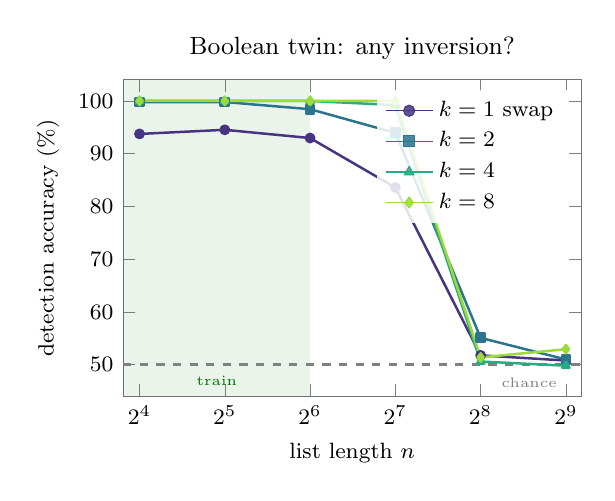
\begin{tikzpicture}
\definecolor{twinA}{RGB}{70,52,128}
\definecolor{twinB}{RGB}{43,116,142}
\definecolor{twinC}{RGB}{37,172,130}
\definecolor{twinD}{RGB}{155,217,60}
\begin{axis}[
  width=7.4cm, height=5.6cm,
  xmode=log, log basis x=2, xmin=14, xmax=580,
  xtick={16,32,64,128,256,512}, xticklabels={$2^4$,$2^5$,$2^6$,$2^7$,$2^8$,$2^9$},
  xlabel={list length $n$}, ylabel={detection accuracy (\%)},
  ymin=44, ymax=104, ytick={50,60,70,80,90,100},
  title={Boolean twin: any inversion?},
  tick label style={font=\footnotesize}, label style={font=\footnotesize},
  title style={font=\small,yshift=-2pt}, axis line style={black!55},
  every axis plot/.append style={line join=round},
  legend cell align=left, legend pos=north east,
  legend style={font=\footnotesize,draw=none,fill opacity=0.85,text opacity=1},
]
\addplot[draw=none,fill=green!45!black,opacity=0.08,forget plot] coordinates {(14,44) (64,44) (64,104) (14,104)} \closedcycle;
\node[font=\tiny,green!45!black] at (axis cs:30,47) {train};
\addplot[gray,dashed,line width=1pt,forget plot] coordinates {(14,50) (580,50)};
\node[font=\tiny,gray] at (axis cs:380,46.5) {chance};
\addplot[twinA,mark=*,mark size=1.5pt,line width=0.9pt,forget plot] coordinates {(16,93.75) (32,94.53) (64,92.97) (128,83.59) (256,51.76) (512,50.78)};
\addplot[twinB,mark=square*,mark size=1.5pt,line width=0.9pt,forget plot] coordinates {(16,99.8) (32,99.8) (64,98.44) (128,93.95) (256,55.08) (512,50.98)};
\addplot[twinC,mark=triangle*,mark size=1.5pt,line width=0.9pt,forget plot] coordinates {(16,100.0) (32,100.0) (64,100.0) (128,99.22) (256,50.59) (512,49.8)};
\addplot[twinD,mark=diamond*,mark size=1.5pt,line width=0.9pt,forget plot] coordinates {(16,100.0) (32,100.0) (64,100.0) (128,100.0) (256,51.37) (512,52.93)};
\addlegendimage{twinA,mark=*}\addlegendentry{$k=1$ swap}
\addlegendimage{twinB,mark=square*}\addlegendentry{$k=2$}
\addlegendimage{twinC,mark=triangle*}\addlegendentry{$k=4$}
\addlegendimage{twinD,mark=diamond*}\addlegendentry{$k=8$}
\end{axis}
\end{tikzpicture}

\caption{The Boolean twin, and where it also runs out. Detection accuracy
for ``is there at least one inversion?'' on lists built with $k$ swaps.
The shaded region is the training range. Detection holds up far longer
than counting does, because its answer stays in $\{0,1\}$ no matter how
long the list gets, which is what makes it intensive. It is worth being
honest that it does eventually fall to chance for small $k$ at the extreme
lengths: a single swap inside a list of $512$ is a very faint signal.
Theorem~\ref{thm:barrier} says nothing about this, since it is a
detectability limit and not a range limit.}
\label{fig:twin}
\end{figure}

So we ran the Boolean twin on the frozen LLM as well, not only in the toy;
Figure~\ref{fig:twin} is the toy version of the same contrast.
Detect asks whether there is any out-of-order pair at all, one bit, against
Count's growing integer. The lists are sorted digit strings, half of them
given $k$ adjacent swaps, and we only ever place a swap where the two neighbours are actually different, because swapping two equal numbers
creates no inversion and a first attempt at this quietly produced almost no positive examples at the longer lengths. Labels come from recomputing
the inversion count, not from trusting the swap count. We report $k \in
\{2,4,8\}$ as the control and hold $k = 1$ out separately, since a single
swap is the faintest possible signal and the margin literature already
predicts trouble there for reasons that have nothing to do with this paper.

The control works, on the mean-pool head. At $n = 48$, reading the same
layer-$14$ states at the same item positions, mean-pool answers Detect
correctly on every list when there are eight swaps and $95.7\%$ of the time
at four. On Count at that same length the same readout reaches $R^2 =
-2.68$, with $0.8\%$ of predictions inside a tenth of the truth and a mean
absolute error of $480$ against a content-blind null of $243$. One readout,
one length, one set of lists, and it answers the bounded question while
doing worse than ignoring the input on the growing one. What separates them
is that the answer grows, not that the list is long.

\begin{table}[htbp]
\centering
\caption{The matched control. Qwen3-0.6B frozen, layer $14$, same item
positions throughout, median over three seeds, chance is $50\%$. Detect is
the bounded target and Count the growing one, on the same lists. Smaller
$k$ means a fainter signal, and $k = 1$ was held out of the control in
advance. The comparison the argument leans on is the $n = 48$ column, where
both were measured.}
\label{tab:twin}
\small
\begin{tabular}{@{}llrrrr@{}}
\toprule
& & $n = 16$ & $n = 32$ & $n = 48$ & $n = 96$ \\
\midrule
Mean-pool, Detect & $k = 8$ & 1.000 & 1.000 & 1.000 & 0.523 \\
(bounded answer) & $k = 4$ & 1.000 & 1.000 & 0.957 & 0.500 \\
 & $k = 2$ & 0.980 & 0.848 & 0.500 & 0.500 \\
 & $k = 1$ & 0.793 & 0.500 & 0.500 & 0.500 \\
\midrule
Mean-pool, Count & $R^2$ & 0.03 & n/a & $-2.68$ & $-3.15$ \\
(growing answer) & within 10\% & 3.9\% & n/a & 0.8\% & 0.0\% \\
\midrule
Value head, Detect & $k = 8$ & 1.000 & 0.500 & 0.500 & 0.500 \\
 & $k = 4$ & 0.949 & 0.500 & 0.500 & 0.500 \\
\bottomrule
\end{tabular}
\end{table}

We wrote down a prediction before running this and it turned out wrong, so
here it is. We expected the value head to hold Detect at $k \ge 2$ all the
way out to $n = 96$. It does not. It is perfect at $n = 16$ with eight
swaps and then sits at chance for every $k$ from $n = 32$ onward, on a
bounded target the theorem says nothing about. That matters for which arm
carries the argument, because for the value head we cannot separate boundedness from a plain failure to generalize in length. The mean-pool arm
can, so the claim rests on that arm now.

The gap between the two arms is itself informative. The value head and the
mean-pool head differ in one respect only, which is where they read. The
value head reads the final token, mean-pool reads the item positions. Same
model, same layer, same target, same lists, and the one reading the items
is still perfect at $n = 48$ while the one reading the last token is at
chance by $n = 32$. That puts the value head's Detect failure in whatever
survives being squeezed into a single final position, which is
over-squashing and is somebody else's result, not ours. It is a second
limitation of the standard readout sitting next to our own, and we would rather point at it than quietly fold it into our own.

For completeness, the tally head itself gets Detect right at essentially
every length and every $k$, including the $k = 1$ corner where both bounded
readouts are at chance, which is unsurprising given that a readout able to
produce the count can also check whether it is positive. Two of three seeds
behave that way and the third is the dead gate again, which we count as a failure and keep in the table. This arm is not part of the control though. The
control compares a bounded readout against two kinds of target, and the
tally head is not bounded, so it sits outside that comparison by
construction.

\subsection{Does a bigger Qwen fix it?}
\label{sec:sizes}
\label{sec:bigger}

A natural objection is that the small Qwen failed because it did not have
enough capacity. We tested a model roughly six to seven times larger.

\begin{table}[htbp]
\centering
\caption{Value-head MAE at $n = 96$, for two base model sizes. The MAE is
almost unchanged.}
\label{tab:sizes}
\begin{tabular}{@{}llr@{}}
\toprule
\textbf{Base model} & \textbf{Size} & \textbf{Value-head MAE at $n=96$} \\
\midrule
Qwen3-0.6B & 0.6 billion parameters & 1{,}992 \\
Qwen3-4B   & 4 billion parameters   & 1{,}972 \\
\bottomrule
\end{tabular}
\end{table}

On the same experiment the MAE is almost the same, which ablates the
capacity objection. With the same one-shot value aggregation, a large
frozen Transformer still cannot reliably output a growing count. This is a
during-validation control.

%=======================================================================

\section{Discussion: Limitations and Conjectures}
\label{sec:discussion}
%=======================================================================

\subsection{Limitations}
\label{sec:limits}

Three limitations bound what this paper shows.

\begin{enumerate}
\item One shared head covering several pairwise rules was not reliable
  across seeds.
\item Pair-sum questions did not learn well from frozen Qwen layer-14
  features.
\item Learned pairwise heads were usually approximate rather than exact.
\end{enumerate}

\subsubsection*{(A) One shared head for several pairwise rules}

We can train a tally head for one pairwise rule at a time, but we cannot
reliably train one shared head to handle several different pairwise rules
selected by the English question.

What succeeded: we trained separate heads, one on inversions only, one on
duplicate pairs, and one on drops of at least five. Each had its own
learned weights and bias.

What did not: we then tried the harder experiment of training a single
shared tally head across ``how many pairs are out of order'', ``how many
duplicate pairs are there'', ``how many pairs drop by at least five'', and
``how many pairs sum to $s$''. The English question is supposed to tell it
which pair rule to use, so the head must switch meaning: for inversions,
earlier value larger than later value; for duplicates, values equal; for
pair-sum, values adding to the target. This is much harder to learn with
one shared bias than with one fixed bias per question type.

The more fundamental reason is gradient interference. When training across
different question types, the gradient from inversion examples pushes the
weights toward ``earlier value bigger'', while the gradient from duplicate
examples pushes toward ``values equal''. At the same time, all the logits
have to sit inside $[0,1]$ for the clamp to learn at all, and even with
active-region initialization, different question types push the logits to
different places.

We tried to tackle this with curriculum training: train each pairwise rule
separately, then aggregate them, then fine-tune. Some pairwise rules
recovered, but others became weaker, and the method could not reliably
handle all of them at once.

The conclusion is that Theorem~\ref{thm:universal} says a suitable
one-head solution exists, but our SGD recipe does not reliably discover it
when several pairwise rules must share a head. This is an optimization
issue, not an expressivity limit, because the architecture can still
express the answer.

\subsubsection*{(B) Pair-sum from frozen Qwen features}

For pair-sum the rule is $P_s(a_j, a_i) = \mathbf{1}[a_j + a_i = s]$, and
its solo-head result was already poor. Even at the training length the
$R^2$ was $0.09$, so the head had barely learned pair-sum \emph{within}
the training range. Therefore its later failure at $n = 96$ is not a clean
extrapolation collapse. With the frozen Qwen features we selected and the
training recipe we used, SGD did not reliably learn the pair-sum
predicate. The learning and implementation did not acquire it, even though
the tally architecture can represent the rule.

\subsubsection*{(C) Learned pairwise heads are approximate, not exact}

For pairwise tasks the head often tracked the count quite well without
landing on the exact integer. At $n = 96$ the tally head $R^2$ is very
close to $1$, but it is not $1$, and the exact-match rate is single-digit:
$0\%$, $1\%$, $3\%$. For item-wise tasks, both $R^2$ and exact match are
relatively high by comparison. The learned pairwise head produces answers
such as $104.2$ when the true inversion count is $100$.

This does not contradict the theorem. The theorem says that for each fixed
rule, suitable exact weights exist. The learned Qwen experiment asks a
different question: can SGD find them, given these frozen Qwen vectors?
Those are quite different questions, and this is the distinction we keep
emphasizing, because it is genuinely important. Something failing does not
mean our tally head aggregation architecture does not work. It may just
mean we hit an optimization or learning limitation.

\subsection{Two conjectures}
\label{sec:conj1}\label{sec:conj2}

\begin{conjecture}[Effective readout scale]
\label{conj:readout}
The 0.6B and 4B models fail alike because their effective readout scales
are alike: the trunk grows, but the final normalized representation and
the learned readout weights sit at the same numerical scale, so the range
of scalar outputs stays the same and both models meet the same barrier.
\end{conjecture}

The evidence is Table~\ref{tab:sizes}, where a $7\times$ larger model
moves the value-head error at $n = 96$ by about one percent. The test is
to multiply the effective output scale by a constant $c$ and check whether
the collapse length moves like $\sqrt{c}$, which would only ever delay the
failure, since any fixed multiple of a finite range is still finite.

\begin{conjecture}[Pairwise predicate accessibility]
\label{conj:access}
A learned tally head extrapolates a pairwise rule only when the frozen
representations make that rule easy for the small comparison head to
distinguish; when the predicate is not recoverable from the hidden states,
no amount of correct summation can recover the count.
\end{conjecture}

The evidence is that pair-sum, the one rule that failed, is also the one
whose item-level probe is weakest (AUC $0.899$ against $0.98$ to $1.00$
elsewhere, Table~\ref{tab:auc}). The test is a dedicated pair probe
$\mathrm{Probe}(h_j, h_i, h_{\text{question}})$, which our item-level
probe cannot substitute for because it asks a different question; probe
accuracy should predict which pairwise rules extrapolate.

%=======================================================================
\section{Conclusion}
\label{sec:conclusion}
%=======================================================================

The main result is a zero-versus-one statement. A standard fixed-depth,
normalized, one-shot Transformer has zero additive heads, and Theorem~\ref{thm:barrier} says it cannot emit any non-trivial
count that grows with list length. Add one un-normalized tally head with
constructed weights, and Theorem~\ref{thm:universal} says it computes any
fixed item-wise or pairwise count in the class exactly. Zero additive
heads suffice for none of these questions. One suffices for all of them.

The barrier depends on very little. Depth, width, positional encoding,
attention sparsity, temperature and numerical precision do not make the
box any bigger, and the box is the whole argument. Every one of those is a knob people
reach for, and none of them enlarges an average. The pigeonhole argument
in Section~\ref{sec:conseq-b} goes through regardless, and the ablation
ladder in Section~\ref{sec:ablation} is the experimental version of the
same point: sharper attention fails, a deeper and wider model fails, and
then removing the denominator, changing nothing else, works.

The experiments say roughly what the theory predicted, though not exactly.
On frozen Qwen features the standard readouts go negative on every question
past the training lengths, meaning they do worse than ignoring the list and
guessing the average, while the small additive head reading those same
features extrapolates on most of them. One shared head taking the question
in plain English answers item-count questions it was never trained on, six
times past its longest training list, and generalizing to ``how many
sevens'' after only ever seeing ``how many threes'' is hard to explain as
memorization.

It is not exact, and we want that stated plainly. The learned pairwise
heads track the count without landing on it: high $R^2$, single-digit exact
match. One shared head covering several pairwise rules at once was not
reliable across seeds, and pair-sum did not learn at all from the layer-14
features we picked, so its failure at long lengths is not even a clean
extrapolation collapse. Theorem~\ref{thm:universal} says suitable weights
exist; it does not say our training recipe finds them. The one place we
could name the mechanism, the dead clamp gate, we fixed, and active-region
initialization turned a fragile four-out-of-eight into eight-out-of-eight.

The main takeaway is the sentence in the title. Softmax answers
\emph{which}. To answer \emph{how many}, the network needs
one wire that is allowed to add, and that wire has to reach the readout
without being normalized on the way. The two aggregators are not competing
for the same job. An additive head is useless as a selector, in exactly
the way softmax is useless for amounts, and a Transformer that has both
can do both.

\paragraph{Future work.} Two things are left open, and both come with an
experiment attached: Conjecture~\ref{conj:readout}, testable by rescaling
the readout and watching where the collapse length moves, and
Conjecture~\ref{conj:access}, testable with a dedicated pair probe. Beyond
the conjectures, three things we have not done. We have not trained the
head jointly with the trunk, where the non-interference argument no longer
applies. We have not measured how much of the reported counting failure in
the wild is tokenization rather than range, which
\citet{zhang2024tokenization} show is not zero. And we have not built the
router that decides when a deployed model should consult the head, which is
where a practical system would live. Whichever way all of that comes out,
the barrier itself does not move, since it was never a claim about
training.

\clearpage
\begin{appendices}

\section{Proofs}
\label{app:proofs}

\subsection{The worst-case-error inequality, step by step}
\label{app:worstcase-deriv}

\paragraph{Step 1: choose two very simple lists.}
Let $n = 10$. The sorted list is
\[
x_{\text{sorted}} = (0,0,0,0,0,1,1,1,1,1),
\]
which has no earlier $1$s before later $0$s, so
$\Inv(x_{\text{sorted}}) = 0$. The maximally unsorted block list is
\[
x^{*} = (1,1,1,1,1,0,0,0,0,0),
\]
where every $1$ is before every $0$, giving $5 \times 5 = 25$ such pairs,
so $\Inv(x^{*}) = 25$. For a general length $n$, splitting the list
roughly in half gives $\Inv(x^{*}) = \lfloor n^2/4 \rfloor$. That is why
the number of inversions grows like $n^2$.

\paragraph{Step 2: the model is trapped inside its output box.}
By Lemma~\ref{lem:bounded}, every prediction lies between $-M(T)$ and
$M(T)$. Call the model's predictions
\[
a = \hat{y}(x_{\text{sorted}}), \qquad b = \hat{y}(x^{*}),
\]
so $a$ is whatever number the model predicts for the sorted list, and $b$
is whatever it predicts for the unsorted, high-entropy list. Therefore
$|a| \leq M(T)$ and $|b| \leq M(T)$. The model may predict different
values for the two lists, but neither prediction can leave this fixed
output range.

\paragraph{Step 3: the error on $x^{*}$ alone.}
For $x^{*}$ the true answer is $I = \lfloor n^2/4 \rfloor$ while the largest
number the model is able to produce is $M(T)$, so its error is
\[
e^{*} \;=\; |b - I| \;\geq\; I - |b| \;\geq\; I - M(T),
\]
which is Eq.~\eqref{eq:worstcase}. With $I = 25$ and $M(T) = 8$, even the
model's best available prediction of $8$ is still off by $17$, so we do not
need a second list to compare it against.

\begin{remark}[The two-list version, and why we keep it]
\label{rem:twolist}
There is a weaker argument that survives on weaker assumptions. Let $a$ and
$b$ be the predictions on $x_{\text{sorted}}$ and $x^{*}$. Walking the route
$0 \rightarrow a \rightarrow b \rightarrow I$ covers at least the direct
distance $I$, and $|b - a| \leq 2M(T)$ because both sit in the box, so
$e_{\text{sorted}} + e^{*} \geq I - 2M(T)$ and at least one of the two is
half of that. It is a factor of two worse. But it never uses $|a| \leq M(T)$
or $|b| \leq M(T)$ on their own, only the width of the box, so if somebody
later builds an architecture whose readout keeps a bounded spread while its
centre drifts with $n$, the single-list argument dies and this one still
gives a quadratic error. The barrier does not care where the box sits, only
that it has a fixed size.
\end{remark}

\subsection{Proof of Theorem~\ref{thm:universal}, pairwise half}
\label{sec:proof-pair}

\paragraph{Step 1: one-hot features.}
Every value in the alphabet gets a one-hot feature vector $f(a)$, which
is a vector of zeros with a single $1$ in the slot for that value. The
only property we need is that the dot product of two one-hot vectors is
$1$ when the values match and $0$ when they do not, so a dot product can
act as a lookup into a table of rules.

\paragraph{Step 3: the universal construction.}
Fix one pair rule $P(\text{earlier value}, \text{later value})$, for
example ``earlier $+$ later $= 2$''. For every possible value $b$ that
appears \emph{later}, define
\begin{equation}
q(b) \;=\; \big(P(0,b),\, P(1,b),\, \dots,\, P(V-1,b)\big),
\label{eq:qb}
\end{equation}
and for every possible value $a$ that appears \emph{earlier}, define
$k(a) = e_a$, the one-hot vector for $a$. Then
\begin{equation}
q(b) \cdot k(a) \;=\; P(a,b),
\label{eq:lookup}
\end{equation}
which is the lookup-table fact.

\paragraph{Step 4: connect it to one actual pair in a list.}
Choose one pair of positions $j < i$. The earlier token has value $a_j$
and the later token has value $a_i$. Substituting $a = a_j$ and $b = a_i$
into Eq.~\eqref{eq:lookup},
\[
q(a_i) \cdot k(a_j) \;=\; P(a_j, a_i),
\]
which is exactly the pair vote we need.

\paragraph{Step 5: write it in standard Transformer notation.}
Queries and keys in a Transformer are produced by weight matrices,
\[
q_i = W_Q f(a_i), \qquad k_j = W_K f(a_j),
\]
where $f(a)$ is the one-hot vector for value $a$. We choose $W_K$ so that
it produces $k(a)$, and $W_Q$ so that it produces $q(a)$. Substituting
into the tally head's score,
\begin{equation}
\big\langle W_Q f(a_i),\, W_K f(a_j) \big\rangle
\;=\; q(a_i) \cdot k(a_j)
\;=\; P(a_j, a_i).
\label{eq:bridge}
\end{equation}

\paragraph{Step 6: add the clamp and the sum.}
Because $P(a_j, a_i)$ is already $0$ or $1$, the clamp leaves it
untouched: $\clampf(P(a_j,a_i), 0, 1) = P(a_j, a_i)$. Therefore
\[
\clampf\big(\langle W_Q f(a_i), W_K f(a_j)\rangle,\, 0,\, 1\big) = P(a_j, a_i),
\]
and summing that equality over every pair with $j < i$,
\begin{equation}
\sum_i \sum_{j<i} \clampf\big(\langle W_Q f(a_i), W_K f(a_j)\rangle, 0, 1\big)
\;=\; \sum_i \sum_{j<i} P(a_j, a_i).
\label{eq:pairhalf}
\end{equation}
The left side is what the tally head computes; the right side is the
definition of the pair count we wanted. \qed

\begin{remark}[What is and is not being claimed]
\label{rem:not-claiming}
For the theorem we can literally write down the tally head's weights
ourselves. We are \emph{not} claiming to know the weights inside a
pretrained Transformer. We only hand-set the small new tally head, for a
rule we already know.
\end{remark}

\begin{example}[``Pairs sum to $2$'', with the actual matrices]
\label{ex:sumto2}
For this rule the table is known:
\[
P = \begin{pmatrix} 0 & 0 & 1 \\ 0 & 1 & 0 \\ 1 & 0 & 0 \end{pmatrix}.
\]
We set $W_K$ to the identity matrix, so a one-hot feature stays the same
as its key, and we set
\[
W_K = \begin{pmatrix} 1&0&0 \\ 0&1&0 \\ 0&0&1 \end{pmatrix},
\qquad
W_Q = \begin{pmatrix} 0&0&1 \\ 0&1&0 \\ 1&0&0 \end{pmatrix}.
\]
Then later value $0$ gets query $(0,0,1)$, selecting earlier $2$; later
value $1$ gets query $(0,1,0)$, selecting earlier $1$; and later value $2$
gets query $(1,0,0)$, selecting earlier $0$. Those are the exact numbers
of the matrices, chosen directly from the rule table.
\end{example}

So the logic is: choose a known rule $P$ $\rightarrow$ write its $0/1$
table $\rightarrow$ turn the table's columns into query vectors
$\rightarrow$ use one-hot keys $\rightarrow$ set $W_Q$ and $W_K$
accordingly $\rightarrow$ the dot product returns the correct answer
exactly. This is why it is called a \emph{constructive} proof: it does not
merely say ``weights probably exist'', it gives a recipe for building
them.

\subsection{Proof of Theorem~\ref{thm:universal}, item-wise half}
\label{sec:proof-item}

Having proved the pairwise counting half, we now solve the item-wise half
for example ``how many $2$s are there in a list?'' The proof is
easier because it does not require the same complexity.

For ``how many $2$s are in the list?'', define
\[
\varphi(a) = \begin{cases} 1 & \text{if } a = 2,\\ 0 & \text{if } a \neq 2.\end{cases}
\]
Using the one-hot idea, for possible values $\Sigma = \{0,1,2\}$ the
one-hot features are $0 \rightarrow (1,0,0)$, $1 \rightarrow (0,1,0)$,
$2 \rightarrow (0,0,1)$. For ``count the $2$s'' define the single vector
$u = (0,0,1)$. Then
\[
u \cdot f(0) = 0, \qquad u \cdot f(1) = 0, \qquad u \cdot f(2) = 1,
\]
so $u \cdot f(a) = \varphi(a)$: the dot product gives the correct $0/1$
vote for each individual item. Summing every item vote gives
$\sum_i \varphi(a_i)$, which is exactly ``how many $2$s?'' \qed

\clearpage
\section{Reproduction Details}
\label{app:repro}

This appendix records the settings needed to rerun everything.

\paragraph{The toy.} The alphabet has $64$ values. Training uses AdamW with
cosine decay and gradient clipping at $1.0$ per tensor, over three seeds,
with $512$ evaluation lists per length. Training lengths run from $8$ to
$64$ and evaluation goes out to $512$; the six-question runs take $8{,}000$
steps. The hand-set column plugs the exact witness weights in and trains
nothing.

\paragraph{Code.} All experiment scripts, figure generators and stored
run outputs are at \texttt{github.com/Co-Messi/Yau-Awards}.

\paragraph{The machine.} Everything ran on one laptop, a MacBook Pro with
an Apple M5 Max, $18$ cores and $64$\,GB of unified memory, under macOS
$26.5$ with Python $3.13.7$ and PyTorch $2.12.0$ on the MPS backend. No
cluster or external GPU was involved. Toy runs take seconds, and the
longest frozen-model run takes minutes.

\paragraph{The frozen model.} The trunk is Qwen3-0.6B-Base, run in float32
on Apple MPS. Each
list item is written as a space followed by one digit, which is exactly two
tokens, so item positions are known by construction, never found by matching
token identities. The question text contains digits too, and matching on
identity would pick those up. Masks are unit tested. The head reads layer $14$ of $28$, LayerNorms what it
reads, and its output bypasses the final LayerNorm on its own wire. The
heads train with AdamW at learning rate $10^{-3}$. Per-question heads train for $1{,}500$ steps, the
shared question-reading head for $8{,}000$. Five seeds for the tally arms and
three for the value head, mean-pool and fraction baselines.

\paragraph{How the lists are built.} Each question has its own sampler,
built so the count does not track the length. Otherwise a model could score
well by reading $n$ and never looking at the contents. Order questions sort, partially reshuffle, then sometimes reverse.
Duplicate questions draw from a random number of distinct values. Sum-to-$s$
plants complementary pairs and fills the rest from a half-set that provably
cannot produce a hit. Item questions plant a uniformly random number of
matches. A check runs before every experiment confirming that the
content-blind guesser scores below $0.2$ on within-ten-percent at every
length. Labels are always recomputed from the list that was actually built,
never assumed from how it was built.

\paragraph{One detail about the evaluation sampler.} Planted samplers draw
the target count first, then build a list realizing it. Two questions given
the same generator seed therefore get the same sequence of counts on
different lists. The two item-family questions in the main tables were
evaluated that way. Labels are still computed from the list they belong to
and each question is still answered on its own inputs, so no number changes.
Read those two columns as two different rules, not two independent draws.
The denominator control, written later, gives each question its own seed
offset.

\paragraph{The figures.} Figures~\ref{fig:scatter}, \ref{fig:collapse},
\ref{fig:twin} and \ref{fig:denominator} are emitted by
\texttt{make\_scatter\_pgf.py}, \texttt{make\_toycollapse\_pgf.py},
\texttt{make\_toytwin\_pgf.py} and \texttt{make\_denominator\_pgf.py}, each
reading its own JSON under \texttt{results/}, so every plotted coordinate
traces back to a stored run. Figure~\ref{fig:sixquestions} is the exception:
\texttt{make\_sixquestions\_pgf.py} carries its twelve values in the script
instead. The six on the right are Table~\ref{tab:shared} in the same order
and can be checked against it. Figure~\ref{fig:aggregators} is a schematic,
and the only raster image here.

\paragraph{The real-document run.} Windows are drawn at random positions in the $329$-row index, not at a
fixed stride, since at $256$ rows a fixed stride makes the twenty windows
near-duplicates of one another. Rows are shuffled inside each window, so
the answer is not fixed by the file's own ordering. We draw twenty windows per
question and length. Scoring was decided before
the first call: take the first integer in the reply, treat a stated range as
its midpoint and flag it, and count a reply with no integer as a non-answer, kept out of the error. Reasoning mode is verified from the reported reasoning-token count, not from the request flag, because one
documented way of switching it off returns a sensible answer while still
running the reasoning underneath.

\section{Full Results on the Frozen Model}
\label{app:qfull}

Every arm and every metric logged for the per-question runs. The tally
column is the per-question head. Value, mean-pool and fraction columns are
medians over three seeds.

\begin{table}[htbp]
\centering
\caption{Every arm and every metric, at $n = 96$, which is six times the
longest training length. ``Corr'' is the fixed-length control, ``w10'' the
fraction of predictions within ten percent, and ``exact'' the fraction
landing on the integer. The last column is what a guesser scores if it
ignores the list and reports the average count for that length.}
\label{tab:qfull}
\small
\begin{tabular}{@{}lrrrrrrrrr@{}}
\toprule
& \multicolumn{5}{c}{\textbf{Additive head}} & \multicolumn{2}{c}{\textbf{$R^2$}} & \multicolumn{2}{c}{\textbf{Fraction head}} \\
\cmidrule(lr){2-6}\cmidrule(lr){7-8}\cmidrule(l){9-10}
\textbf{Question} & $R^2_{16}$ & $R^2_{96}$ & corr & w10 & exact & value & mean & $R^2_{96}$ & exact \\
\midrule
How many out of order & 1.00 & 0.96 & 0.99 & 84\% & 3\% & $-3.2$ & $-3.1$ & 0.80 & 0\% \\
How many drop by $\ge 5$ & 0.85 & 0.79 & 0.96 & 12\% & 1\% & $-2.4$ & $-2.3$ & $-0.64$ & 0\% \\
How many duplicate pairs & 0.98 & 0.95 & 0.98 & 35\% & 0\% & $-1.7$ & $-1.7$ & 0.95 & 0\% \\
How many pairs sum to $s$ & 0.09 & $-1.93$ & 0.45 & 4\% & 0\% & $-0.9$ & $-0.9$ & $-0.91$ & 0\% \\
How many equal $v$ & 1.00 & 1.00 & 1.00 & 99\% & 98\% & $-1.8$ & $-1.7$ & 0.88 & 2\% \\
How many above $c$ & 1.00 & 1.00 & 1.00 & 100\% & 79\% & $-2.2$ & $-1.8$ & 0.83 & 2\% \\
\bottomrule
\end{tabular}
\end{table}

Three things in it the main text has no room for.

The within-ten-percent column separates two kinds of success that $R^2$ runs
together. On the two item counts the head is right, not just correlated:
$99\%$ and $100\%$ within a tenth, most of them on the integer. On
out-of-order pairs it tracks the count well, $R^2 = 0.96$ and correlation
$0.99$, but lands within ten percent only $84\%$ of the time and on the
integer $3\%$. Both are real. They are not the same result.

The fraction head shows the second wall cleanly. It is the rescale-by-$n$
escape: predict a bounded ratio, multiply by the number of pairs outside the
model. On three questions it reaches $R^2$ of $0.80$, $0.95$ and $0.88$, and
on those same three it is exact $0\%$, $0\%$ and $2\%$. That is the signature
the theory predicts. Dividing escapes the range wall and lands straight into
a resolution one, since neighbouring counts are now about $2/(n(n-1))$ apart
on a channel with finite precision.

The last column rules out the cheap explanation. Ignoring the list and
guessing the typical count for that length scores $0$ to $14$ percent on
within-ten-percent. The additive head scores $84$ to $100$ on four of the
six.

\end{appendices}

\clearpage
\bibliographystyle{plainnat}
\bibliography{refs}

\clearpage
\section*{Acknowledgements}
\addcontentsline{toc}{section}{Acknowledgements}

\subsection*{Research background, and the advising relationship}

The question originally came from a meme: even frontier models like GPT
sometimes cannot say how many r's are in the word strawberry. That is the
old folklore meme. When I was first introduced to large language models I
thought this was about maturity and parameter count, and that the
technology simply had not improved enough. As time went on I came to
realize it is an architecture issue rather than a size issue, and that got
me intrigued enough to want to solve it properly and, if possible, give an
adequate fix. I later learned that the strawberry case itself is mostly a
tokenization problem, which is exactly why every experiment in this paper
uses clean single-digit tokens, so the deeper failure can be seen on its
own.

With some knowledge of Transformers, linear algebra and large language
models, I began exploring. At first all I understood was that attention is
bounded, without being able to say how it stays bounded as the input grows
forever. The inspiration for the fix came while I was studying
convolutional neural networks, and this is the part I want to emphasize.
In a CNN the kernels detect edges and patterns by taking a dot product
against the input and looking at the size of the response. That made me
ask whether the same move could be generalized to the counting problem:
make the goal a one-hot vector, treat every token in the vocabulary as
another vector, take dot products and sum them up, which is basically a
feature map in a convolutional network. After that comes the clamp gate,
which plays the role ReLU plays in a CNN. That is how everything started.
Using what I knew about backpropagation and gradient descent, I then
applied learning methods to fit the weights of the whole system and
generalize.

My advisors are Dr.\ Junaid Khan and Mr.\ Liang Ren. \needwrite{How each
advising relationship came about, and what each advisor contributed at
which stage.} All guidance from both advisors was unpaid throughout. Apart
from my advisors, no one else assisted with this work; the research and
the writing were done independently.

\subsection*{Division of work, and difficulties met}

I was the sole student author. The topic came from the observation above
and was narrowed over several months of testing candidate weaknesses. I
wrote the samplers that generate all the synthetic data, and built the
real-document benchmark from a public index of past award entries. All
analysis, computation and experiments were designed and run by me, on the
single laptop described in Appendix~\ref{app:repro}, and I wrote the
paper. \needwrite{What each advisor contributed at which stage, one or
two sentences each.}

Several problems came up along the way. The clamp gate has zero gradient
outside its active band, and early training
runs died with every vote stuck at $0$ or at $1$; the fix, active-region
initialization, came only after tracing the failures seed by seed. The
first data generator for the detection control quietly produced almost no
positive examples at long lengths, because swapping equal neighbours
creates no inversion, and it had to be rebuilt around strict ascents. A
prediction I wrote down before running the detection control came out
wrong, which changed which experimental arm the argument rests on. And in
the real-document run, an ambiguous wording of ``pairs'' confounded two
early sessions, which were discarded and rerun with the question spelled
out.

\subsection*{Declaration on the use of AI tools}

At the very beginning I used two tools, the ChatGPT and DeepSeek
websites, and I used them to gather papers. Once the papers were
gathered, I read every abstract myself, wrote a brief summary of each,
worked out the current status of the problem and where its limitation
sits, and proposed the solution myself. I then handed the proposal back
to the AI to check whether it was doable, and after that to my advisors,
who told me I could go and try.

From then on the working pattern was the one my advisors warned me about:
the first attempt always fails, in the code or in the hypothesis, and my
job was to diagnose from first principles why. I would diagnose it myself
first, then give my thought process to the AI to look for what I had
missed, then run the ablations.
Auditing and diagnosing code was where AI help was most efficient, and it
was also useful when searching for related ideas. Later in the project I
used Claude as a coding and writing assistant: it wrote and debugged
experiment scripts under my direction, generated the figures from the
stored run outputs, and helped draft and edit the LaTeX of this paper,
always working from my results, outlines and instructions. The DeepSeek
model tested inside the paper (DeepSeek-V4-Pro, called through its API)
is an experimental subject, not an assistant. All experimental numbers
come from code run on the machine described in Appendix~\ref{app:repro},
and I checked the reported tables against the raw outputs myself.

Throughout, I also used AI as a learning partner: I would ask it
questions in a Socratic way, make it explain the project back to me, and
keep questioning until the explanation either broke or held, which is also
how several bugs were diagnosed. These tools were used from roughly June
to September 2026.
\needwrite{Rough frequency of use (the upload form asks for 使用时间及频率
and 名称及版本, so add versions here too if you are willing).} AI was a
good companion and collaborator throughout, but all of the thinking and
all of the original ideas came from me. I do not believe AI can create the
new solution for me.
Both advisors approved this use of AI tools in advance.

\end{document}
